\chapter{LANDASAN TEORI}

\section{Tinjauan Pustaka}


    Dalam penelitian ini, beberapa teori dasar 
    akan digunakan untuk memberikan penjelasan 
     lebih komprehensif terhadap proses penelitian 
     dan mendalami pemahaman terkait dengan topik 
     yang diadopsi. Untuk mendukung metodologi 
     penelitian ini, beberapa sumber referensi 
     akan digunakan sebagai acuan untuk mengkaji 
      konsep dasar pengolahan citra digital, 
      pengenalan gambar dalam bentuk objek digital, 
      serta metode yang digunakan. Metode penelitian 
       dipilih yaitu \textit{Convolutional Neural Network}  (CNN) akan 
       dijelaskan secara rinci pada bagian selanjutnya. Metode CNN 
       digunakan dikarena pendekatan ini merupakan jenis 
       teknik \textit{neural network} yang secara khusus dibuat 
       untuk mengatasi masalah pada data dua dimensi (2D) yang terdiri 
       dari berbagai ukuran piksel \cite{Lindholm2022}. Beberapa 
       mengenai deteksi kantuk dapat dilihat pada Tabel \ref{Tabel Perbandingan Referensi} berikut.

    

      \begin{table}[H]
        \centering
        \caption{Penelitian Mengenai Deteksi Kantuk}
         \label{Tabel Perbandingan Referensi}
        \begin{tabular}%{p{0.5cm}p{1.8cm}p{2.9cm}p{1.1cm}p{4.1cm}p{1cm}}
              {  >{\raggedright\arraybackslash}p{0.3cm} 
        >{\raggedright\arraybackslash}p{2.0cm} 
        >{\raggedright\arraybackslash}p{2.5cm} 
        >{\raggedright\arraybackslash}p{1.5cm} 
        >{\raggedright\arraybackslash}p{4.0cm} 
        >{\raggedright\arraybackslash}p{0.9cm}}
    
            \hline
            \textbf{No} & \textbf{Penulis} & \textbf{Topik} &\textbf{ Metode} & \textbf{Hasil} & \textbf{Tahun} \\
            
            \hline
             1 
            & 
            Fiaz Majeed, Umair Shafique, Mejdl Safran, Sultan Alfarhood, and Imran Ashraf
            &
            \textit{Detection of Drowsiness among Drivers Using Novel Deep Convolutional Neural Network Model}
            & 
            CNN \& RNN
            &
            Hasil eksperimen menunjukkan bahwa model yang diusulkan mencapai akurasi rata-rata 96,69\% tanpa augmentasi data, yang lebih unggul dari yang sudah ada yang sudah ada dalam mendeteksi kantuk.
            &
            2023 \\  
            \\

             2 
            & 
            Ruben Florez, Facundo Palomino-Quispe, Roger Jesus Coaquira-Castillo, Julio Cesar, Thuanne and Ana Beatriz
            & 
            \textit{A CNN-Based Approach for Driver Drowsiness Detection by Real-Time Eye State Identification}
            & 
            CNN
            &
            Dari 10 percobaan yang dilakukan dan menunjukkan hasil akurasi yang tinggi dalam mendeteksi kantuk menggunakan CNN berdasaran tiga arsitektur  yaitu InceptionV3, VGG16 dan ResNet50V2. Dengan akurasi masing-masing sebesar 99.31\%, 99.41 \%, dan 99.71\%. 
            &
            2023 \\
                \hline

        \end{tabular}
    \end{table}




         \begin{table}[H]
        \centering
        \begin{tabular}%{p{0.5cm}p{1.8cm}p{2.9cm}p{1.1cm}p{4.1cm}p{1cm}}
        {>{\raggedright\arraybackslash}p{0.3cm} 
        >{\raggedright\arraybackslash}p{2.0cm} 
        >{\raggedright\arraybackslash}p{2.5cm} 
        >{\raggedright\arraybackslash}p{1.5cm} 
        >{\raggedright\arraybackslash}p{4.0cm} 
        >{\raggedright\arraybackslash}p{0.9cm}}
    
            \hline
            \textbf{No} & \textbf{Penulis} & \textbf{Topik} &\textbf{ Metode} & \textbf{Hasil} & \textbf{Tahun} \\    
            \hline

            3 
            & 
            Hepatika Zidny Ilmadina, Dyah Apriliani, Dega Surono Wibowo
            &
            Deteksi Pengendara Mengantuk dengan Kombinasi Haar 
                \textit{Cascade Classifier} dan \textit{Support Vector Machine}
            &
            SVM \& KNN
            &
            Berdasarkan percobaan yang telah dilakukan diperoleh evaluasi untuk SVM untuk \textit{accuracy} 0.99, \textit{precision} 0.99, dan recall 0.99 dan untuk KNN \textit{accuracy} 0.97, \textit{precision} 0.89, dan \textit{recall} 0.99. Berdasarkan data tersebut dapat disimpulkan bahwa performa yang baik dicapai oleh model SVM dibandingkan dengan KNN.
            &
            2020 \\
            \\
        
                4
            &
            Venkata Rami Reddy Chirra1, Srinivasulu Reddy, Venkata Krishna Kishore
            &
            \textit{Deep CNN: A Machine Learning Approach for Driver Drowsiness Detection Based on Eye State}
            &
            CNN
            &
            Dari 1200 sampel latih, 1150 sampel uji dan 500 sampel validasi, diperoleh  akurasi latih sebesar 98\%. Akurasi validasi 97\% dan akurasi uji 96.42\%.

            &

            2019 \\
            \\

             5
            & 
            Tereza Soukupova and Jan ´Cech &
           \textit{ Real-Time Eye Blink Detection using Facial Landmarks} &
            EAR SVM &

           Pada deteksi \textit{landmarks} kesalahan cukup kecil hingga 5\% dari IOD tetapi untuk \textit{interface} kesalahan di bawah 10\%. Pada deteksi kedipan akurasi tetap tinggi hingga rata-rata IOD sekitar 30 px.
             &
            2017\\

             \hline

        \end{tabular}
    \end{table}



        


       
\section{Kecelakaan}

    Menurut Undang-Undang (UU) Republik Indonesia Pasal 1 No. 22 tahun 2009, kecelakaan lalu lintas dapat diartikan sebagai peristiwa yang terjadi di jalan raya secara tiba-tiba dan tidak disengaja, melibatkan kendaraan atau pengguna jalan lainnya, dan berakibat pada korban jiwa atau kerusakan harta benda. Kondisi kantuk dapat menjadi salah satu faktor yang menyebabkan kecelakaan lalu lintas. Kantuk dapat mengurangi kewaspadaan dan reaksi pengemudi, sehingga meningkatkan risiko terjadinya kecelakaan. Selain itu, kelelahan juga dapat menjadi penyebab utama terjadinya kantuk saat berkendara. Faktor-faktor lain yang dapat menyebabkan kecelakaan lalu lintas meliputi kelalaian pengguna jalan, kondisi kendaraan yang tidak layak jalan, kondisi jalan yang tidak memadai, serta kondisi lingkungan seperti cuaca buruk atau jalan yang licin \cite{Utomo2023}.
    

\section{Kantuk}
    Kantuk merupakan keadaan di mana seseorang merasa ingin tidur. Biasanya,
     kondisi ini disertai dengan mata yang terasa berat dan sulit 
     berkonsentrasi. Kantuk seringkali ditandai dengan keadaan menguap. 
     Ini adalah respons fisiologis yang umum terjadi pada manusia. 
     Ketika seseorang merasa kantuk, otak dapat mengirim sinyal 
     untuk mengurangi kejernihan dan kewaspadaan. Salah satu tanda-tanda 
     menguap sering kali disertai dengan membuka mulut lebar \cite{CALDWELL2019272}. Kantuk merupakan gejala dari kelelahan yang dipengaruhi oleh waktu dan mekanisme homeostasis dalam tubuh.
     
    Homeostasis adalah mekanisme yang menjaga keseimbangan internal tubuh, termasuk dalam hal tidur dan bangun. Keadaan ini biasanya terjadi pada malam hari saat tubuh secara alami merasa lebih siap untuk tidur, namun juga dapat terjadi pada siang hari akibat kurangnya tidur atau perubahan jam tidur yang eksternal. Meskipun kantuk pada siang hari dianggap wajar, tetapi dapat menjadi masalah jika terjadi saat berkendara atau melakukan aktivitas lain yang memerlukan kewaspadaan \cite{Puspasari2023}.
    Rasa kantuk dapat mengakibatkan berbagai masalah, termasuk menghambat 
    produktivitas di tempat kerja, memengaruhi emosi, dan menyebabkan 
    kecelakaan, baik di jalan maupun di tempat kerja. Meskipun rasa 
    mengantuk adalah hal yang biasa, jika terjadi secara tidak normal, 
    hal ini mungkin mengindikasikan gejala penyakit. Seperti sleep apnea, 
    narkolepsi, insomnia, depresi, gangguan kecemasan, atau 
    diabetes \cite{Susanto2020}.

    Akibat merasakan kantuk, seseorang bisa mengalami \textit{microsleep}, yaitu keadaan hilang kesadaran. Peristiwa ini biasanya terjadi selama 1 detik hingga 2 menit. \textit{Microsleep} terjadi karena aktivitas yang monoton, seperti menatap layar komputer terus menerus atau berkendara dalam waktu yang cukup lama. Teori ini digunakan sebagai acuan untuk mendeteksi kondisi kantuk berdasarkan kondisi mata. Apabila mata tertutup kurang dari 3 detik, berarti keadaan tidak mengantuk. Namun, jika mata tertutup lebih dari 3 detik, pengendara sedang mengantuk \cite{puteri2020deteksi}.

\section{\textit{Computer Vision}}

    \textit{Computer Vision} adalah bidang dalam ilmu komputer yang berkonsentrasi pada pembuatan algoritma untuk memberdayakan komputer dalam memahami gambar dan video \cite{Guntara2023}. \textit{Computer Vision }telah berkembang di berbagai domain, mencakup kegiatan seperti menangkap data mentah dan mengekstraksi pola dari gambar untuk menginterpretasikan informasi. \textit{Computer Vision} menggabungkan berbagai metode, prinsip, dan konsep yang berasal dari pemrosesan citra digital, pengenalan pola, kecerdasan buatan, dan grafik komputer. Mayoritas tugas dalam \textit{computer vision} berkisar pada perolehan informasi tentang suatu peristiwa atau deskripsi dari masukan gambar digital, termasuk ekstraksi fitur \cite{Noerifanza2022}. 


    \textit{Computer Vision} diidentifikasi sebagai disiplin ilmu dengan seperangkat teknik yang bertujuan untuk memungkinkan komputer memahami konten gambar digital. Bidang multidisiplin ini sebagian besar dibangun di atas konsep pembelajaran mesin, yang menggabungkan algoritma pembelajaran yang terus berkembang. Tujuan utamanya adalah mengembangkan sistem otomatis yang mampu mengekstraksi informasi dari gambar digital yang diberikan.  Deskripsi mengenai \textit{computer vision}, seperti yang diilustrasikan pada Gambar \ref{Konsep Dasar Computer Vision} \cite{Guntara2023} berikut.


    \begin{figure}[H]
        \centering
        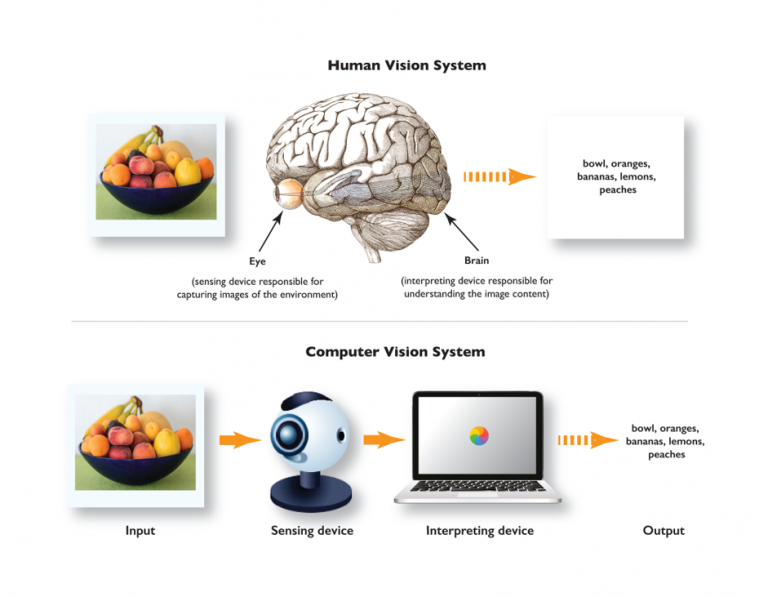
\includegraphics[width=0.7\textwidth]{figures/bab2/computer vision.jpg}
        \caption{Ilustrasi \textit{Computer Vision} \cite{ideas}}
        \label{Konsep Dasar Computer Vision}
    \end{figure}


   


\section{Pengolahan Citra Digital}

    Pemrosesan gambar digital dibagi menjadi tiga tingkatan yang berbeda sebagai berikut: 

    \begin{enumerate}
    
        \item  Tingkat rendah, melibatkan operasi mendasar pada gambar digital, termasuk tugas-tugas seperti akuisisi gambar, dan merekayasa kualitas gambar. Hal ini dicapai melalui tindakan seperti peningkatan kontras, pengurangan atau penambahan \textit{noise}, dan penajaman gambar.

        \item  Tingkat menengah, pemrosesan komputer mencakup operasi yang lebih rumit dalam menangani gambar, khususnya mengubah ukuran, memotong, dan segmentasi. Tingkat pemrosesan ini memiliki hasil yang berbeda dari proses tingkat yang lebih rendah, karena proses ini mengambil data gambar sebagai masukan dan menghasilkan informasi berbeda yang telah diekstraksi secara efektif dari gambar. Informasi yang diekstraksi ini mungkin mencakup fitur seperti kontur, deteksi tepi, dan detail relevan lainnya.

        \item Tingkat tinggi, di mana pemrosesan gambar diarahkan untuk mengidentifikasi objek dalam gambar yang diberikan. Tahap ini  melibatkan pembelajaran mesin, klasifikasi, dan berbagai algoritma kecerdasan buatan.

    \end{enumerate}
    
    
    
  Untuk pemahaman yang lebih mendalam mengenai perkembangan pada setiap tahap pemrosesan gambar digital, berikut representasi visual yang ditunjukkan pada Gambar \ref{Proses Dalam Pengolahan Citra Digital} berikut ini.


    \begin{figure}[H]
    \centering
    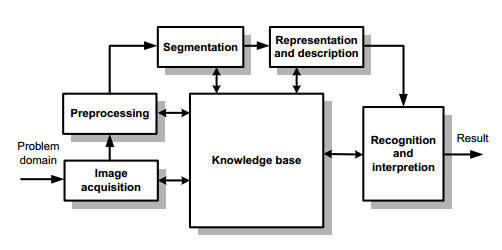
\includegraphics[width=0.75\textwidth]{figures/bab2/Block-diagram.jpg}
    \caption{Proses Pengolahan Citra Digital \cite{sathiya2017novel}}
    \label{Proses Dalam Pengolahan Citra Digital}
\end{figure}

    

    Tujuan pemrosesan gambar digital adalah menghasilkan gambar berkualitas tinggi, memfasilitasi ekstraksi informasi yang mudah, baik oleh manusia maupun mesin.
    Teknik dalam pengolahan citra juga dapat digunakan untuk mentrasformasikan citra digital menjadi sebuah citra lain \cite{Kirana2021}.  

\subsection{Citra Digital}

    Citra digital merupakan representasi gambar dua dimensi menggunakan satu set nilai digital tertentu,
     yang sering disebut sebagai piksel atau elemen gambar. Citra terdiri dari $m \times n$ piksel, di mana setiap
      piksel diwakili oleh $k$ bit. Sebuah piksel, dilambangkan dengan $k$-bit, memiliki $2^k$ corak berbeda dalam
       gambar skala abu-abu. Nilai piksel ini biasanya terdiri dari bilangan bulat dalam rentang 0
        (mewakili piksel hitam) hingga $(2^k - 1)$ (mewakili piksel putih). Besaran nilai piksel ini 
        memainkan peran penting dalam menentukan resolusi dan mempengaruhi kualitas gambar secara 
        keseluruhan \cite{book}. Nilai yang menentukan intensitas gambar atau derajat skala abu-abu atau warna 
         suatu gambar dinyatakan sebagai fungsi dari intensitas gambar, dilambangkan dengan $f(x, y)$. Hal ini
          muncul dari representasi suatu gambar sebagai matriks dua dimensi, seperti yang digambarkan
           pada Gambar \ref{Sistem Koordinat Matematis Sebuah Citra} \cite{Andono2018} berikut.

    \begin{figure}[H]
      \centering
      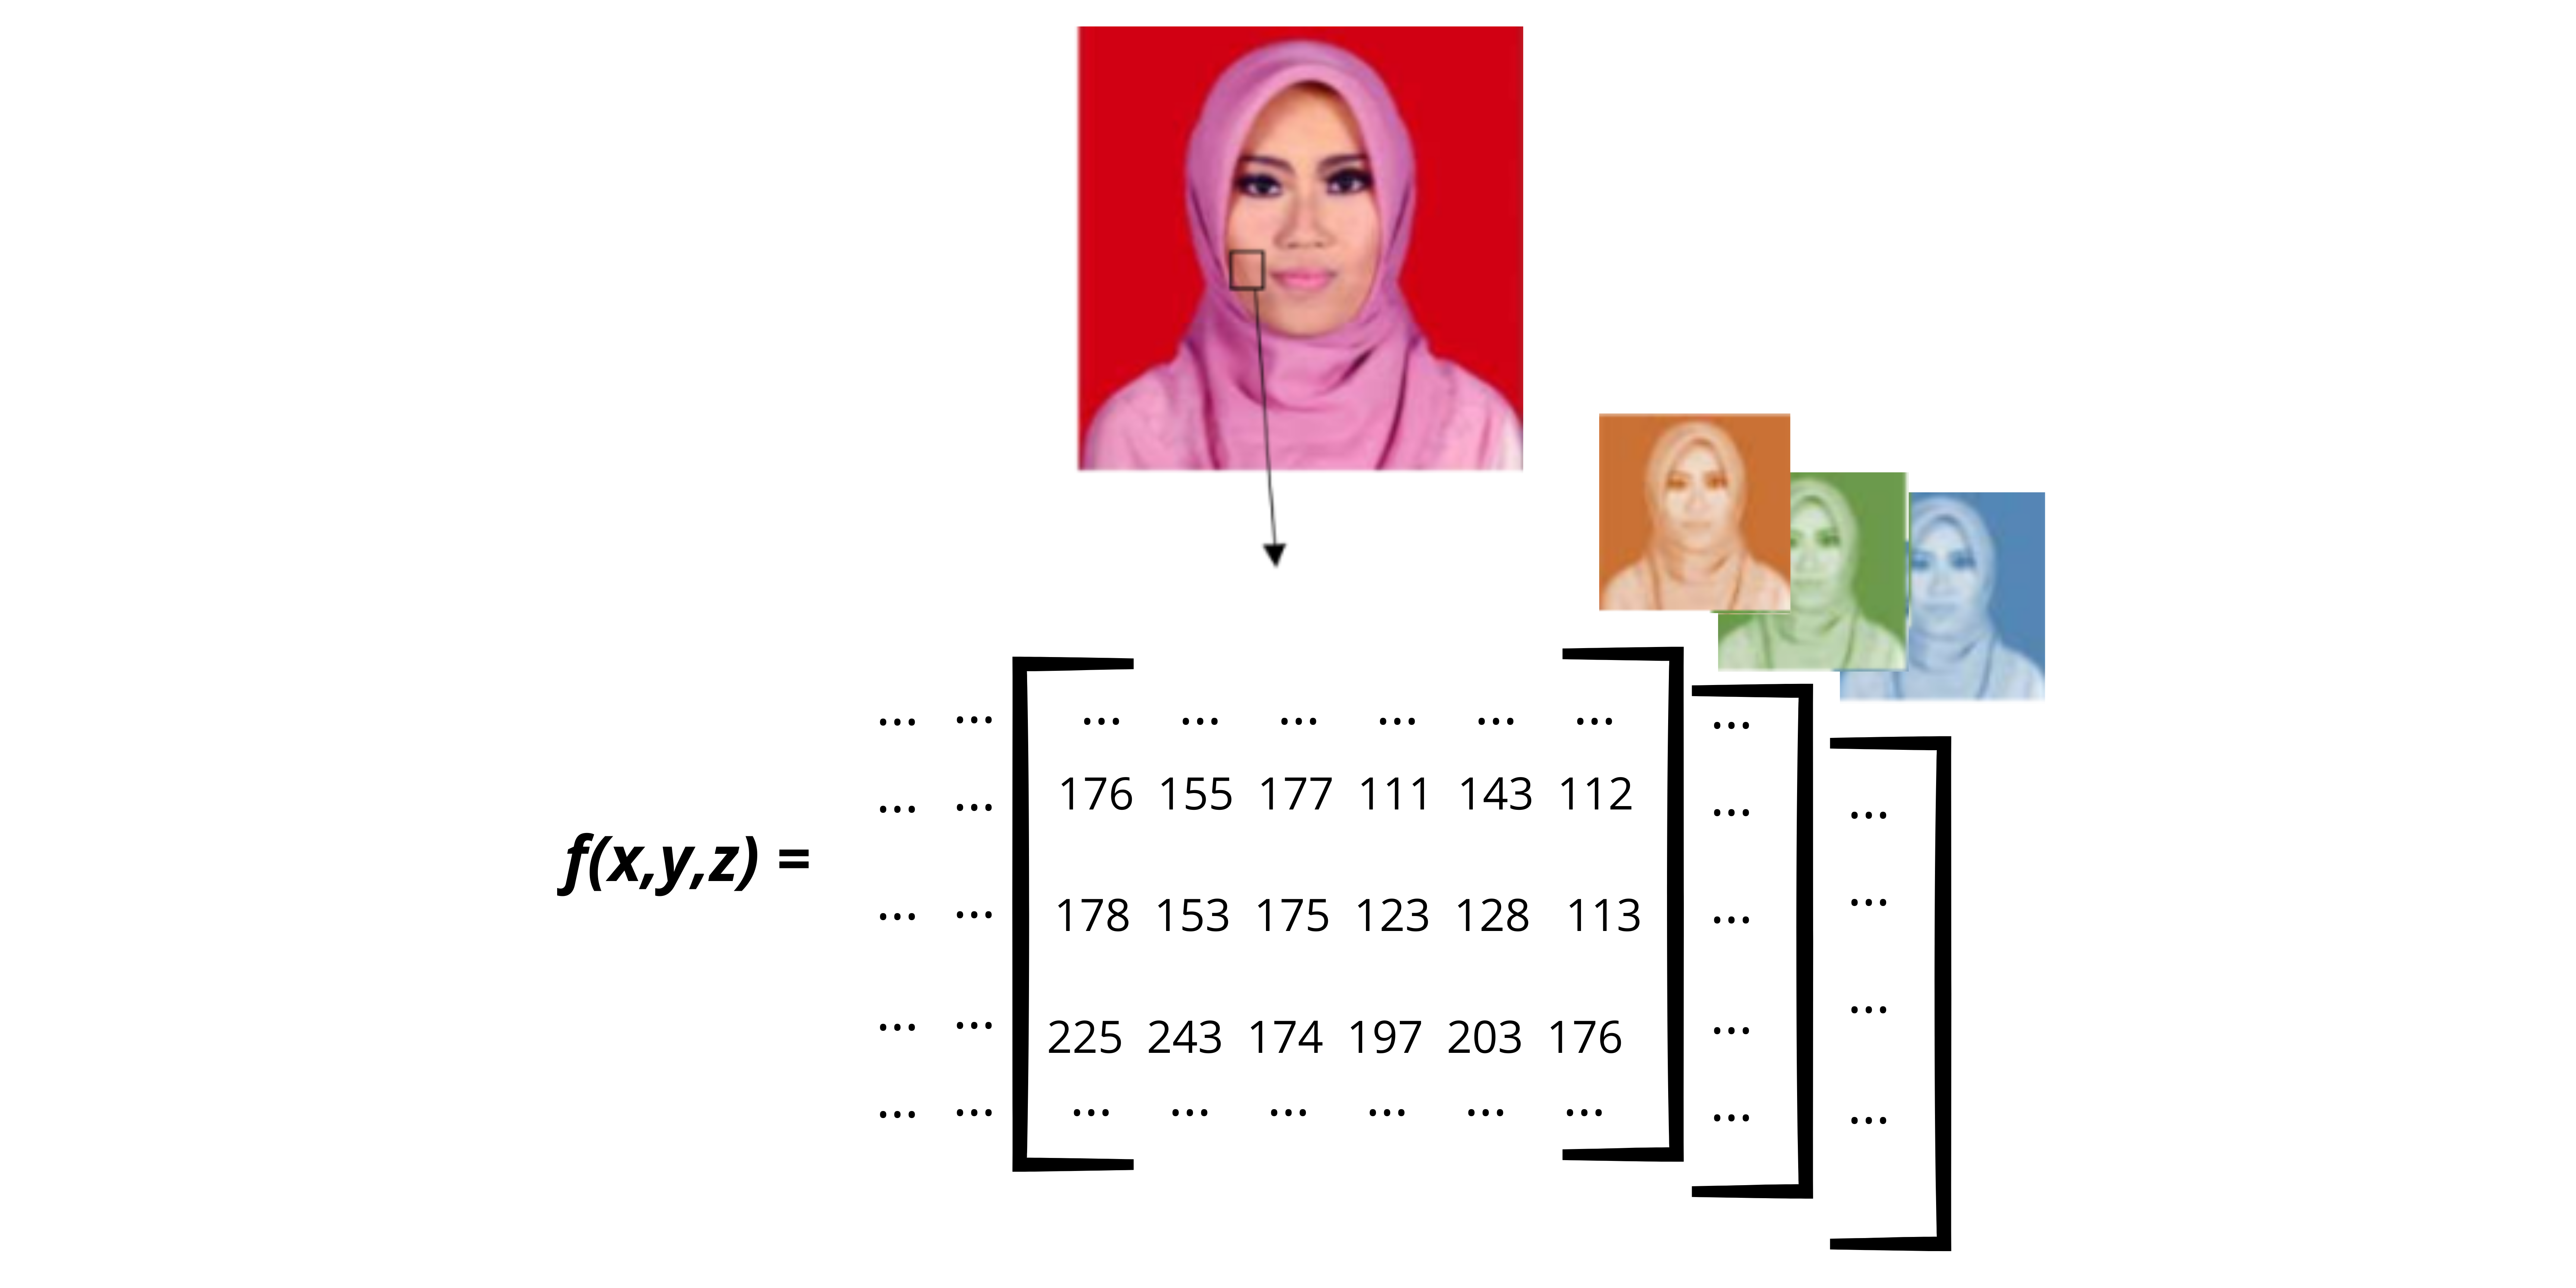
\includegraphics[width=0.85\textwidth]{figures/bab2/citra_digital.png}
      \caption{Sistem Koordinat Matematis Sebuah Citra \cite{Kirana2021}}
      \label{Sistem Koordinat Matematis Sebuah Citra}
    \end{figure}




    
    
    Pada Gambar \ref{Sistem Koordinat Matematis Sebuah Citra} memberikan visualisasi bentuk wajah seorang manusia 
    dengan warna kulit sawo matang dan kerudung pink. Visualisasi wajah manusia tersebut merupakan sebuah kombinasi
     pixel yang membuat intensitas warna yang di tunjukkan pada fungsi $f(x,y)$. Berdasarkan persamaan tersebut, $f$ 
     diasumsikan sebagai intensitas warna dan $(x,y,z)$ adalah koordinat pada dimensi x dan y pada \textit{layer} z yang menjadi chanel warna. 
     Sehingga citra sering didefenisikan sebagai sebuah fungsi yang memuat kombinasi intensitas warna dengan koordinat
      tertentu \cite{Kirana2021}.

\subsection{Akuisisi Citra  Digital}

    Dalam pemrosesan gambar digital, persyaratan awal adalah objek gambar digital itu sendiri. Hal ini dicapai melalui langkah akuisisi gambar, di mana gambar digital diperoleh dengan menggunakan alat akuisisi seperti kamera digital, ponsel pintar, mesin pemindai, internet, dll. Alat-alat ini menghasilkan kumpulan data dalam format seperti JPG, PNG, Bitmap, atau yang serupa. Tahap ini juga disebut sebagai tahap pengumpulan dataset \cite{Dewi2018}.
    
    
    Langkah awal lingkungan ditangkap menggunakan sebuah sensor electronik citra yag terbuat dari sensor cahaya CCD \textit{(charge-coupe device}) atau CMOS \textit{(Complementary Metal Oxide Semiconductor)}. Kemudian sensor elektronik mengubah intensitas cahaya dan frekuensi menjadi sebuah gelombang analog. Gelombang analog yang dihasilkan tersebut akan diubah menjadi sinyal digital \cite{putra2010pengolahan}.

\subsection{Augmentasi Citra }

    Augmentasi gambar digital bertujuan untuk memperluas jumlah kumpulan data yang tersedia. Hal ini dilakukan untuk meningkatkan keragaman data tanpa memerlukan proses akuisisi berulang, yang biasanya memakan waktu dan biaya mahal. Salah satu praktik umum dalam proses augmentasi citra digital melibatkan transformasi bentuk data awal yang diperoleh melalui proses akuisisi. Modifikasi yang potensial mencakup memutar gambar digital saat ini pada berbagai sudut, mengubah ruang warna, memperkenalkan \textit{noise}, serta menerjemahkan dan memotong gambar. Tujuannya adalah untuk mencegah \textit{overfitting}, di mana model secara berulang-ulang mengidentifikasi fitur yang sama selama tahap-tahap selanjutnya dari proses pelatihan. Pendekatan ini bertujuan untuk meningkatkan kinerja model ketika ditugaskan untuk mengenali data uji. Ilustrasi augmentasi gambar digital dapat dilihat pada Gambar \ref{Contoh Augmentasi Citra} berikut \cite{Shorten2019, shorten2019survey}.

    
    \begin{figure}[H]
      \centering
      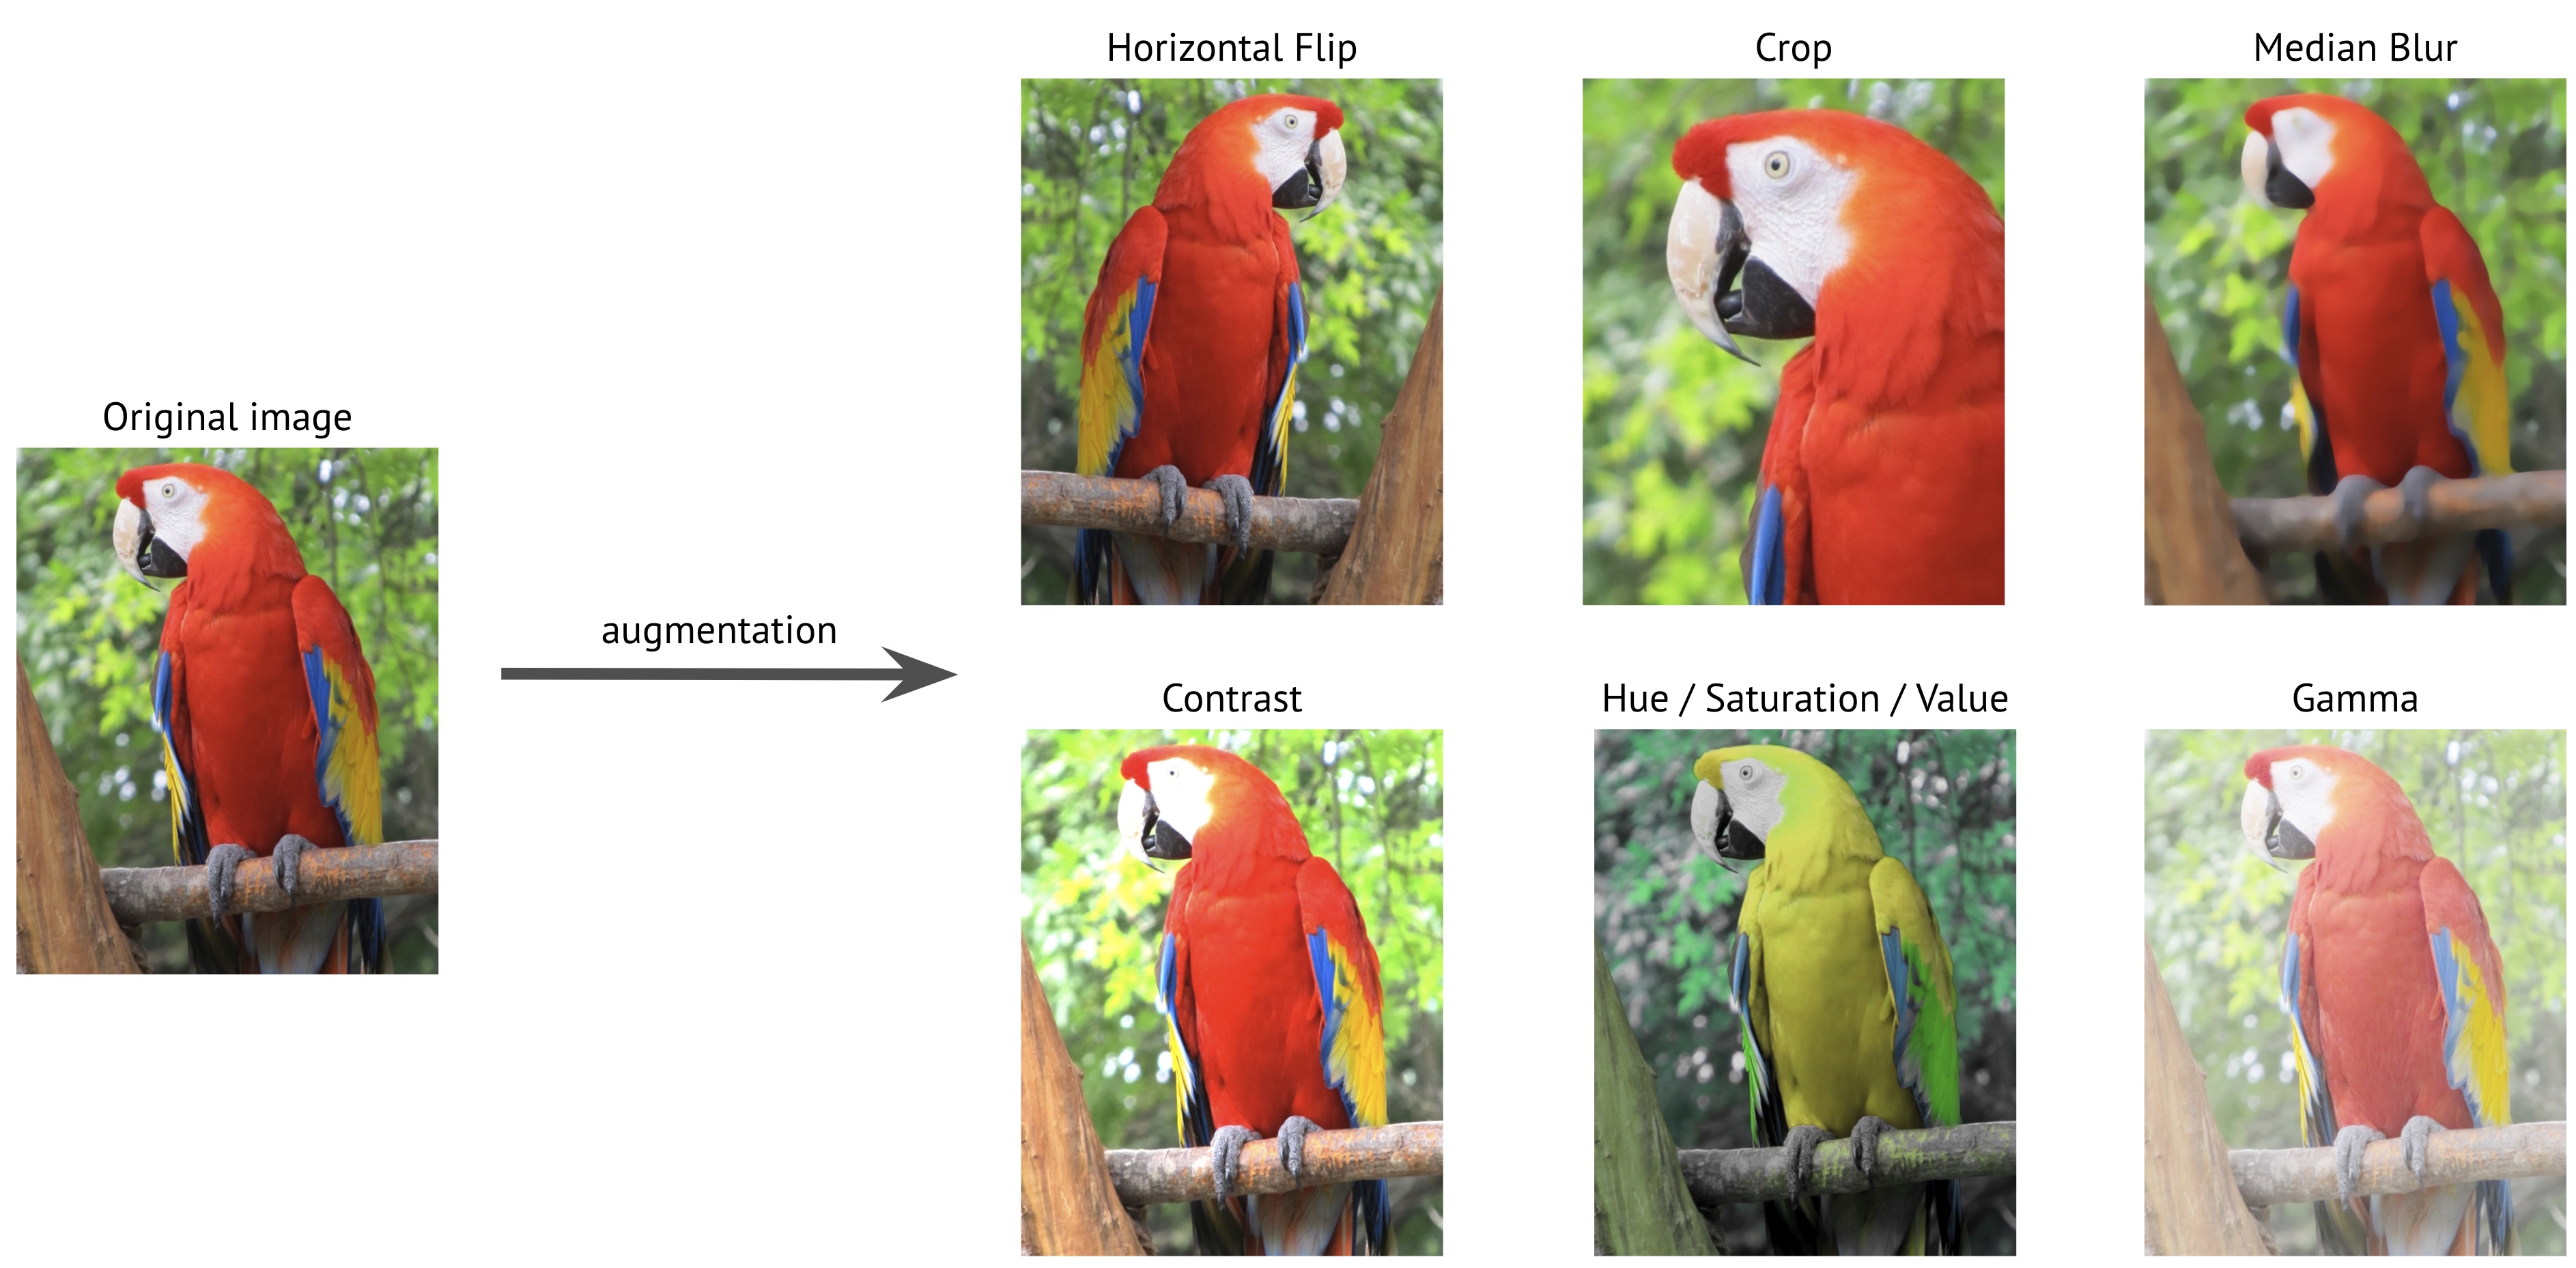
\includegraphics[width=0.85\textwidth]{figures/bab2/augmentation.jpg}
      \caption{Contoh Augmentasi Citra \cite{info11020125}}
      \label{Contoh Augmentasi Citra}
    \end{figure}


    Untuk lebih detail terkait metode-metode augmentasi dijabarkan sebagai berikut

    \subsubsection{\textit{Affine} Transformation}

    
        Dengan menggunakan pendekatan ini, matriks transformasi \textit{affine} dikalikan dengan matriks gambar yang diproses. Transformasi ini menonjol karena kemampuannya untuk mempertahankan bidang, titik, dan garis lurus yang terlihat pada gambar asli. Untuk augmentasi geometris, transformasi \textit{affine} sering digunakan untuk operasi seperti rotasi, translasi, pergeseran, dan penskalaan/pembesaran. Hal ini dimungkinkan karena Persamaan \ref{Affine Transformation} menerapkan gambar yang disediakan \cite{Gonzalez2009}.

   

        \begin{equation}
         \begin{aligned}
            \begin{vmatrix}
                x' \\
                y' \\
                1 \\
            \end{vmatrix} = A \begin{vmatrix}
                x \\
                y \\
                1 \\
            \end{vmatrix} = \begin{vmatrix}
                \alpha_{11} & \alpha_{12} & t_x \\
                \alpha_{21} & \alpha_{22} & t_y \\
                0 & 0 & 1 \\
            \end{vmatrix} \begin{vmatrix}
                x \\
                y \\
                1 \\
            \end{vmatrix}
            \end{aligned} \label{Affine Transformation}
        \end{equation}


        \begin{itemize}
            \item $\alpha_{11}$ dan $\alpha_{22}$ menunjukkan faktor skala untuk sumbu x dan y. Parameter ini mengatur perubahan ukuran objek.

            \item  $\alpha_{21}$ dan $\alpha_{12}$ mewakili rotasi atau \textit{shearing}. Jika  $\alpha_{12} \neq 0$, maka objek akan mengalami rotasi terhadap sumbu x. Sebaliknya, jika $\alpha_{21} \neq 0$, objek akan mengalami rotasi terhadap sumbu y.

            \item $t_x$ dan $t_y$ menunjukkan translasi (geseran) dalam arah x dan y. Parameter ini menentukan seberapa jauh objek digeser dari posisi awalnya.

            \item Baris ketiga $(0,0,1)$ merupakan baris tetap yang memungkinkan representasi vektor homogen (tipe vektor yang dapat mewakili koordinat titik dalam ruang homogen).

            
        \end{itemize}

    
        

        Untuk melakukan augmentasi gambar geometris secara komprehensif, berbagai jenis matriks transformasi \textit{affine} digunakan untuk menyesuaikan augmentasi sesuai dengan persyaratan tertentu. Matriks transformasi \textit{affine} yang sesuai dengan masing-masing teknik, termasuk rotasi, \textit{translation, shearing, zooming} dirinci dalam Tabel  \ref{Matriks Transformasi Afin pada Operasi Lainnya}.
        
\begin{table}[H]
    \centering
    \caption{Matriks Transformasi \textit{Affine}}
    \label{Matriks Transformasi Afin pada Operasi Lainnya}
    %\scriptsize
    \begin{tabular}{
        >{\raggedright\arraybackslash}m{1.0cm} 
        >{\centering\arraybackslash}m{3.5cm} 
        >{\raggedright\arraybackslash}m{4.5cm}  
        >{\centering\arraybackslash}m{3.0cm}}
        \hline
        \textbf{Teknik} & \textbf{Matriks} & \textbf{Keterangan} & \textbf{Hasil} \\
        \hline \\
        Translasi & 
        \(\begin{bmatrix}
            1 & 0 & 0 \\
            0 & 1 & 0 \\
            t_x & t_y & 1 \\
        \end{bmatrix}\)
        
        & 
        
        Nilai $t_x$ mewakili pergeseran citra sepanjang sumbu $x$, sedangkan nilai $t_y$ mengindikasikan perpindahan citra sepanjang sumbu $y$.
        
        &
        
     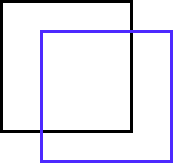
\includegraphics[width=2.0cm, height=2.0cm, keepaspectratio]{figures/bab2/translasi} \\
        
        \textit{Zooming}
        
        & 
        
        \(\begin{bmatrix}
            s_x & 0 & 0 \\
            0 & s_y & 0 \\
            0 & 0 & 1 \\
        \end{bmatrix}\) &
        $s_x$ menunjukkan perubahan skala citra sepanjang sumbu $x$, sementara $s_y$ menggambarkan perubahan skala citra sepanjang sumbu $y$. &
        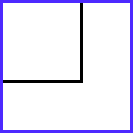
\includegraphics[width=2.0cm, height=2.0cm, keepaspectratio]{figures/bab2/zoom.png} \\
        \\
        
        \textit{Shear} & 
        \(\begin{bmatrix}
            1 & sh_y & 0 \\
            sh_x & 1 & 0 \\
            0 & 0 & 1 \\
        \end{bmatrix}\) &
        $sh_x$ adalah nilai skala untuk pergeseran citra sepanjang sumbu $x$, sementara $sh_y$ adalah nilai skala untuk pergeseran citra sepanjang sumbu $y$. &
        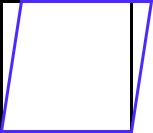
\includegraphics[width=2.0cm, height=2.0cm, keepaspectratio]{figures/bab2/shear.png} \\
        
        \textit{Rotation} & 
        \(\begin{bmatrix}
            \cos \theta & \sin \theta & 0 \\
            -\sin \theta & \cos \theta & 0 \\
            0 & 0 & 1 \\
        \end{bmatrix}\) &
        $\theta$ adalah besar sudut perputaran citra. &
        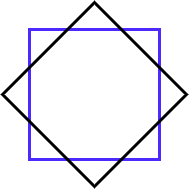
\includegraphics[width=2.0cm, height=2.0cm, keepaspectratio]{figures/bab2/rotasi} \\ 

        \\
        \hline
    \end{tabular}
\end{table}




   

\subsubsection{\textit{Brightness} Dan \textit{Contrast}}

    Praktik membuat gambar dan memodifikasi kecerahan dan kontras untuk setiap gambar baru dikenal sebagai meningkatkan 
    nilai kecerahan dan kontras gambar. Karena dapat meningkatkan performa pengenalan gambar pada model, strategi 
    augmentasi ini sering digunakan dalam penelitian terkait pembelajaran mesin \cite{mikolajczyk2018data, Yang2022}. 
    Ada beberapa metode untuk menerapkan kedua modifikasi ini. Salah satu metode untuk meningkatkan tingkat kecerahan 
    adalah dengan mengubah gambar RGB menjadi HSV, yang memisahkan tiga saluran warna (h, s, dan v). 
    Saluran \textit{value} (v) nilainya berkisar antara $-50 < v < 50$ yang mengontrol kecerahan gambar,
     \textit{saturation} (s) mengukur intensitas atau kemurnian warna dan \textit{hue} (h) merepresentasikan jenis warna yang dirasakan manusia, seperti merah, hijau, biru, kuning, dll. Gambar segar dengan kecerahan yang diubah dihasilkan dengan mengubah saluran v yang dimodifikasi kembali menjadi RGB seperti Gambar \ref{Contoh Augmentasi Contrast} \cite{oza2020empirical, Stollnitz1996}.

    \begin{figure}[H]
      \centering
      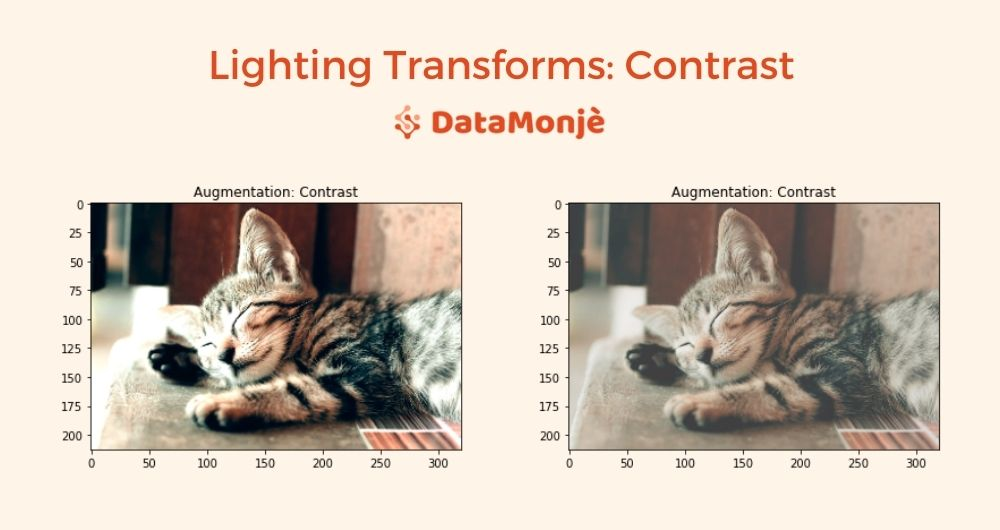
\includegraphics[width=0.75\textwidth]{figures/bab2/Lighting-Transforms-Contrast-augmentation.jpg}
      \caption{Contoh Augmentasi \textit{Brightness} dan\textit{ Contrast} \cite{anand}}
      \label{Contoh Augmentasi Contrast}

    
     \end{figure} 
    
    Berbagai teknik, termasuk penyesuaian kontras linier, mengubah skala nilai piksel individual, 
    menggunakan metode berbasis histogram, dan teknik berbasis resonansi, dapat digunakan untuk 
    mengubah nilai kontras gambar melalui augmentasi \cite{Bebis2021, Maragatham2015, szeliski2021computer}. 
    Teknik sederhana yang dapat digunakan untuk mengontrol nilai kontras pada suatu gambar dapat dilakukan dengan 
    Persamaan \ref{Augmentasi Nilai Kontras} sebagai berikut.

    
    
    \begin{equation}
      \begin{aligned} 
        g(i, j) = \alpha \cdot f(i, j) + \beta
        \end{aligned}\label{Augmentasi Nilai Kontras}
    \end{equation}


    \textbf{Keterangan:}
      \begin{align*}
        f(x) & : \text{Nilai probabilitas densitas fungsi (PDF) pada titik } x. \\
        g(i, j) & : \text{Nilai piksel pada gambar yang diubah (\textit{output})}. \\
        \alpha & : \text{Faktor kontras}. \\
         f(i, j) & : \text{Nilai piksel pada gambar asli (\textit{input})}.\\
         \beta & : \text{Nilai bias}.\\
    \end{align*}

    Persamaan ini merepresentasikan proses perkalian dan penjumlahan dua buah titik dengan sebuah konstanta. 
    Parameter \textit{gain} dan \textit{bias}, dilambangkan dengan $\alpha$ dan  $\beta$, menentukan nilai kontras 
    dan kecerahan masing-masing \cite{Szeliski2021}.
    
\subsubsection{\textit{Gaussian Noise}}


     Dengan menggunakan persamaan distribusi normal (juga dikenal sebagai distribusi Gauss dalam Persamaan \ref{Rumus Distribusi Normal (Gaussian)}). Gaussian diterapkan untuk menyempurnakan gambar dengan menambahkan \textit{noise}. Dengan menggunakan metode ini, nilai piksel gambar digital diubah. Dalam kasus tertentu, menambahkan \textit{noise} gaussian ke pengenalan atau klasifikasi gambar memberikan perkiraan model yang mendekati fitur skenario dunia nyata yang sedang dipelajari.
 

    \begin{equation}
        \begin{aligned}
            f(x) = \frac{1}{\sigma \sqrt{2\pi}} \exp\left(-\frac{1}{2} \left(\frac{x - \mu}{\sigma}\right)^2\right)
        \end{aligned}\label{Rumus Distribusi Normal (Gaussian)}
    \end{equation}


    \textbf{Keterangan:}
      \begin{align*}
        f(x) & : \text{Nilai probabilitas densitas fungsi (PDF) pada titik } x \\
        \sigma & : \text{Standar deviasi distribusi} \\
        \pi & : \text{Konstanta matematika pi dengan nilai } \pi \approx 3.14\\
        \mu & : \text{Rata-rata distribusi} \\
        \exp & : \text{Fungsi eksponensial} \\
        x & : \text{Nilai variabel acak yang ingin dihitung probabilitasnya} \\
    \end{align*}
    


    
    Variabel x mewakili intensitas nilai yang akan didistribusikan, $\mu$ adalah nilai mean dari distribusi tersebut, dan $\sigma$ adalah standar deviasi dari nilai baru yang dimasukkan ke dalam distribusi citra awal.



\section{\textit{Eye Aspect Ratio} (EAR)}

    Pendeteksian \textit{Eye Aspect Ratio }(EAR) merupakan metode yang digunakan untuk mengukur keterbukaan mata. EAR dihitung dengan menggunakan rasio jarak antara beberapa \textit{landmark} mata \cite{electronics11193183}. Dapat dilihat pada Persamaan \ref{rumus ear} berikut.

    
    \begin{equation}
    \label{rumus ear}
    (\text{EAR}_{\text{left}}, \text{EAR}_{\text{right}}   = \frac{{\| \vec{p}_2 - \vec{p}_6 \| + \| \vec{p}_3 - \vec{p}_5 \|}}{{2 \| \vec{p}_1 - \vec{p}_4 \|}})
    \end{equation}

    \begin{equation}
    \text{EAR} = \frac{1}{2}(\text{EAR}_{\text{left}} + \text{EAR}_{\text{right}})
    \end{equation}


    \textbf{Keterangan:}
    \begin{align*}
        \vec{p}_i & : \text{Vektor posisi dari titik ke-i} \\
        \|\vec{p}_2 - \vec{p}_6\| & : \text{Jarak antara titik } \vec{p}_2 \text{ dan } \vec{p}_6 \\
        \|\vec{p}_3 - \vec{p}_5\| & : \text{Jarak antara titik } \vec{p}_3 \text{ dan } \vec{p}_5 \\
        \|\vec{p}_1 - \vec{p}_4\| & : \text{Jarak antara titik } \vec{p}_1 \text{ dan } \vec{p}_4 \\
    \end{align*}
    

    Pada persamaan EAR dijelaskan diatas, di mana $\vec{p}_1$ hingga $\vec{p}_6$ mewakili lokasi
     \textit{landmark 2D} pada retina. $\vec{p}_2, \vec{p}_3, \vec{p}_5,$ dan $\vec{p}_6$ digunakan 
     untuk mengukur tinggi mata, sedangkan $\vec{p}_1$ dan $\vec{p}_4$ digunakan untuk mengukur lebar mata. 
     Saat mata tertutup, nilai EAR dengan cepat turun hingga hampir nol, berbeda dengan saat mata terbuka, 
     yang nilai EARnya tetap konstan. Hal ini digambarkan pada Gambar \ref{Ilustrasi Perhitungan Nilai EAR} berikut.

    \begin{figure}[H]
      \centering
      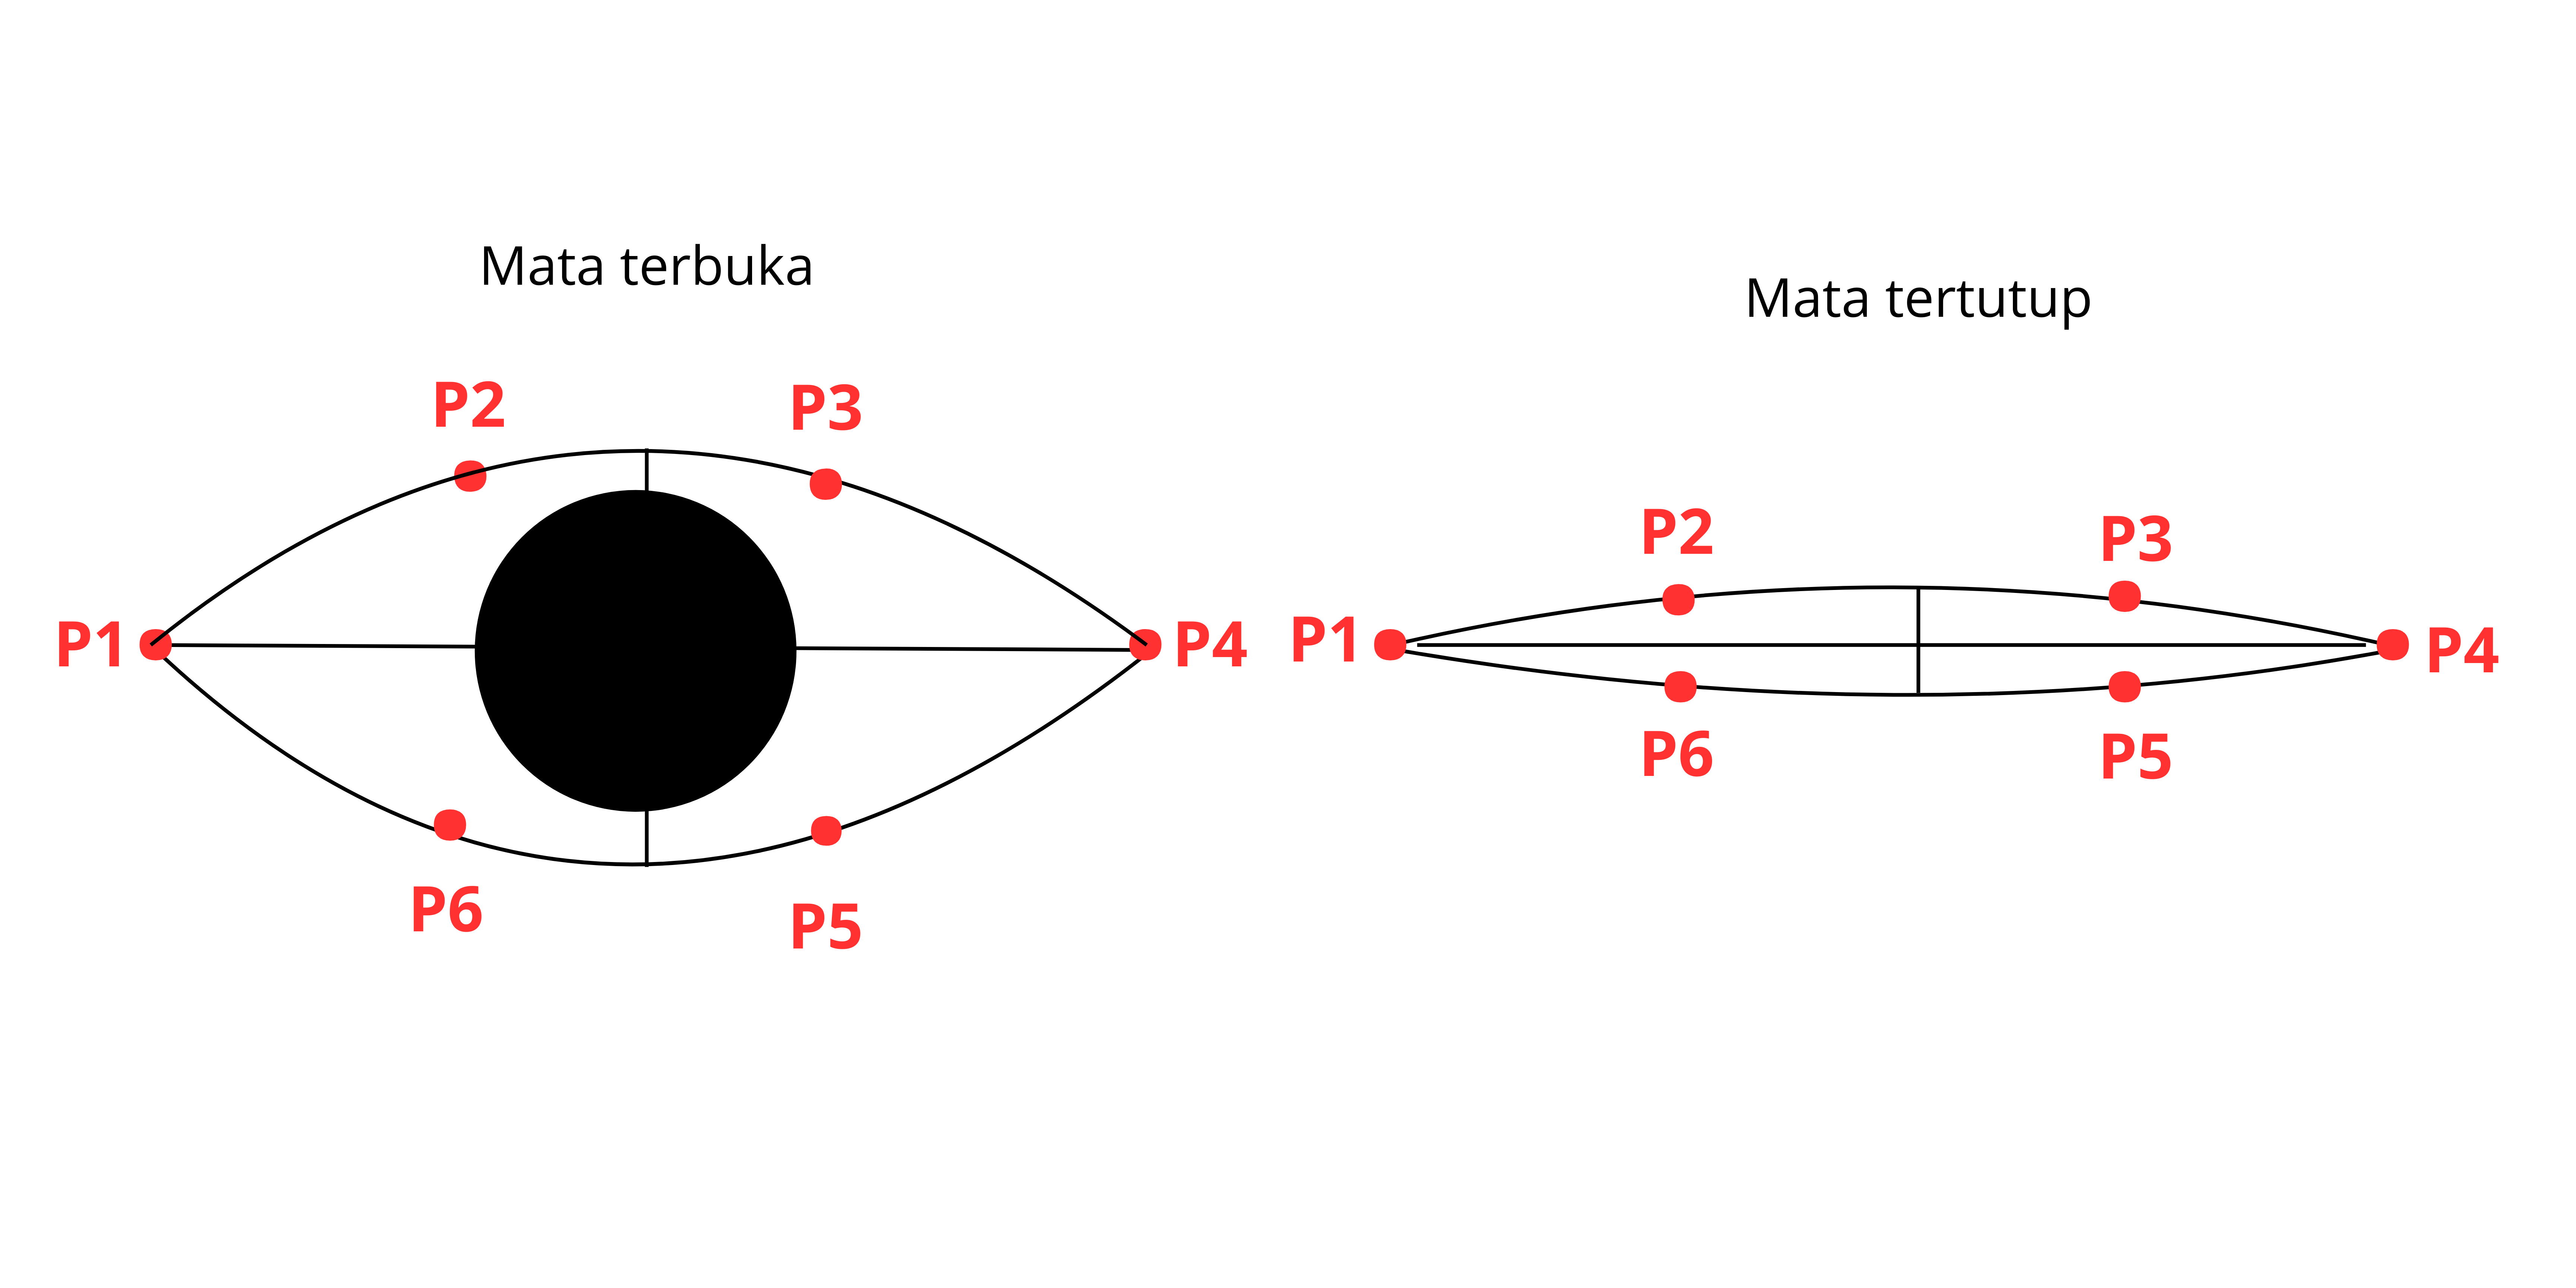
\includegraphics[width=0.8\textwidth]{figures/bab2/EAR.png}
      \caption{Ilustrasi Perhitungan Nilai EAR}
      \label{Ilustrasi Perhitungan Nilai EAR}
    \end{figure}
    
     untuk mengukur tingkat kesalahan deteksi yang terjadi. Tingkat kesalahan deteksi dapat memberikan informasi berharga mengenai akurasi dalam mengidentifikasi kondisi yang benar. Kesalahan deteksi dapat dihitung menggunakan Persamaan \ref{rumus error} berikut.


    \begin{equation}
        \label{rumus error}
        \begin{aligned}
        \text{\textit{error}} = \left(\frac{\text{FP}}{\text{TP + FP}}\right) \times 100\%
        \end{aligned}
    \end{equation}

       \textbf{Keterangan:}
      \begin{align*}
        TN & : \text{Benar melakukan prediksi} \\
        FN & : \text{Salah melakukan prediksi} \\
    \end{align*}

   

\section{\textit{Mouth Aspect Ratio} (MAR)}

Pendeteksian \textit{Mouth Aspect Ratio} (MAR) merupakan metode yang digunakan untuk mengukur lebar terbuka mulut. MAR dihitung dengan menggunakan rasio jarak antara beberapa \textit{landmark} mulut. Koordinat digunakan untuk mewakili mulut. Dimulai dari
sudut kiri mulut, yang tengara ditandai dalam searah jarum jam di sekitar sisanya
wilayah tersebut. MAR diukur dengan membagi vertikal jarak antara bibir atas dan bibir bawah dengan horizontal jarak antara kedua bibir \cite{inproceedings, jimaging9050091}. Dapat dilihat pada Persamaan \ref{rumus mar} berikut.


    \begin{figure}[H]
      \centering
      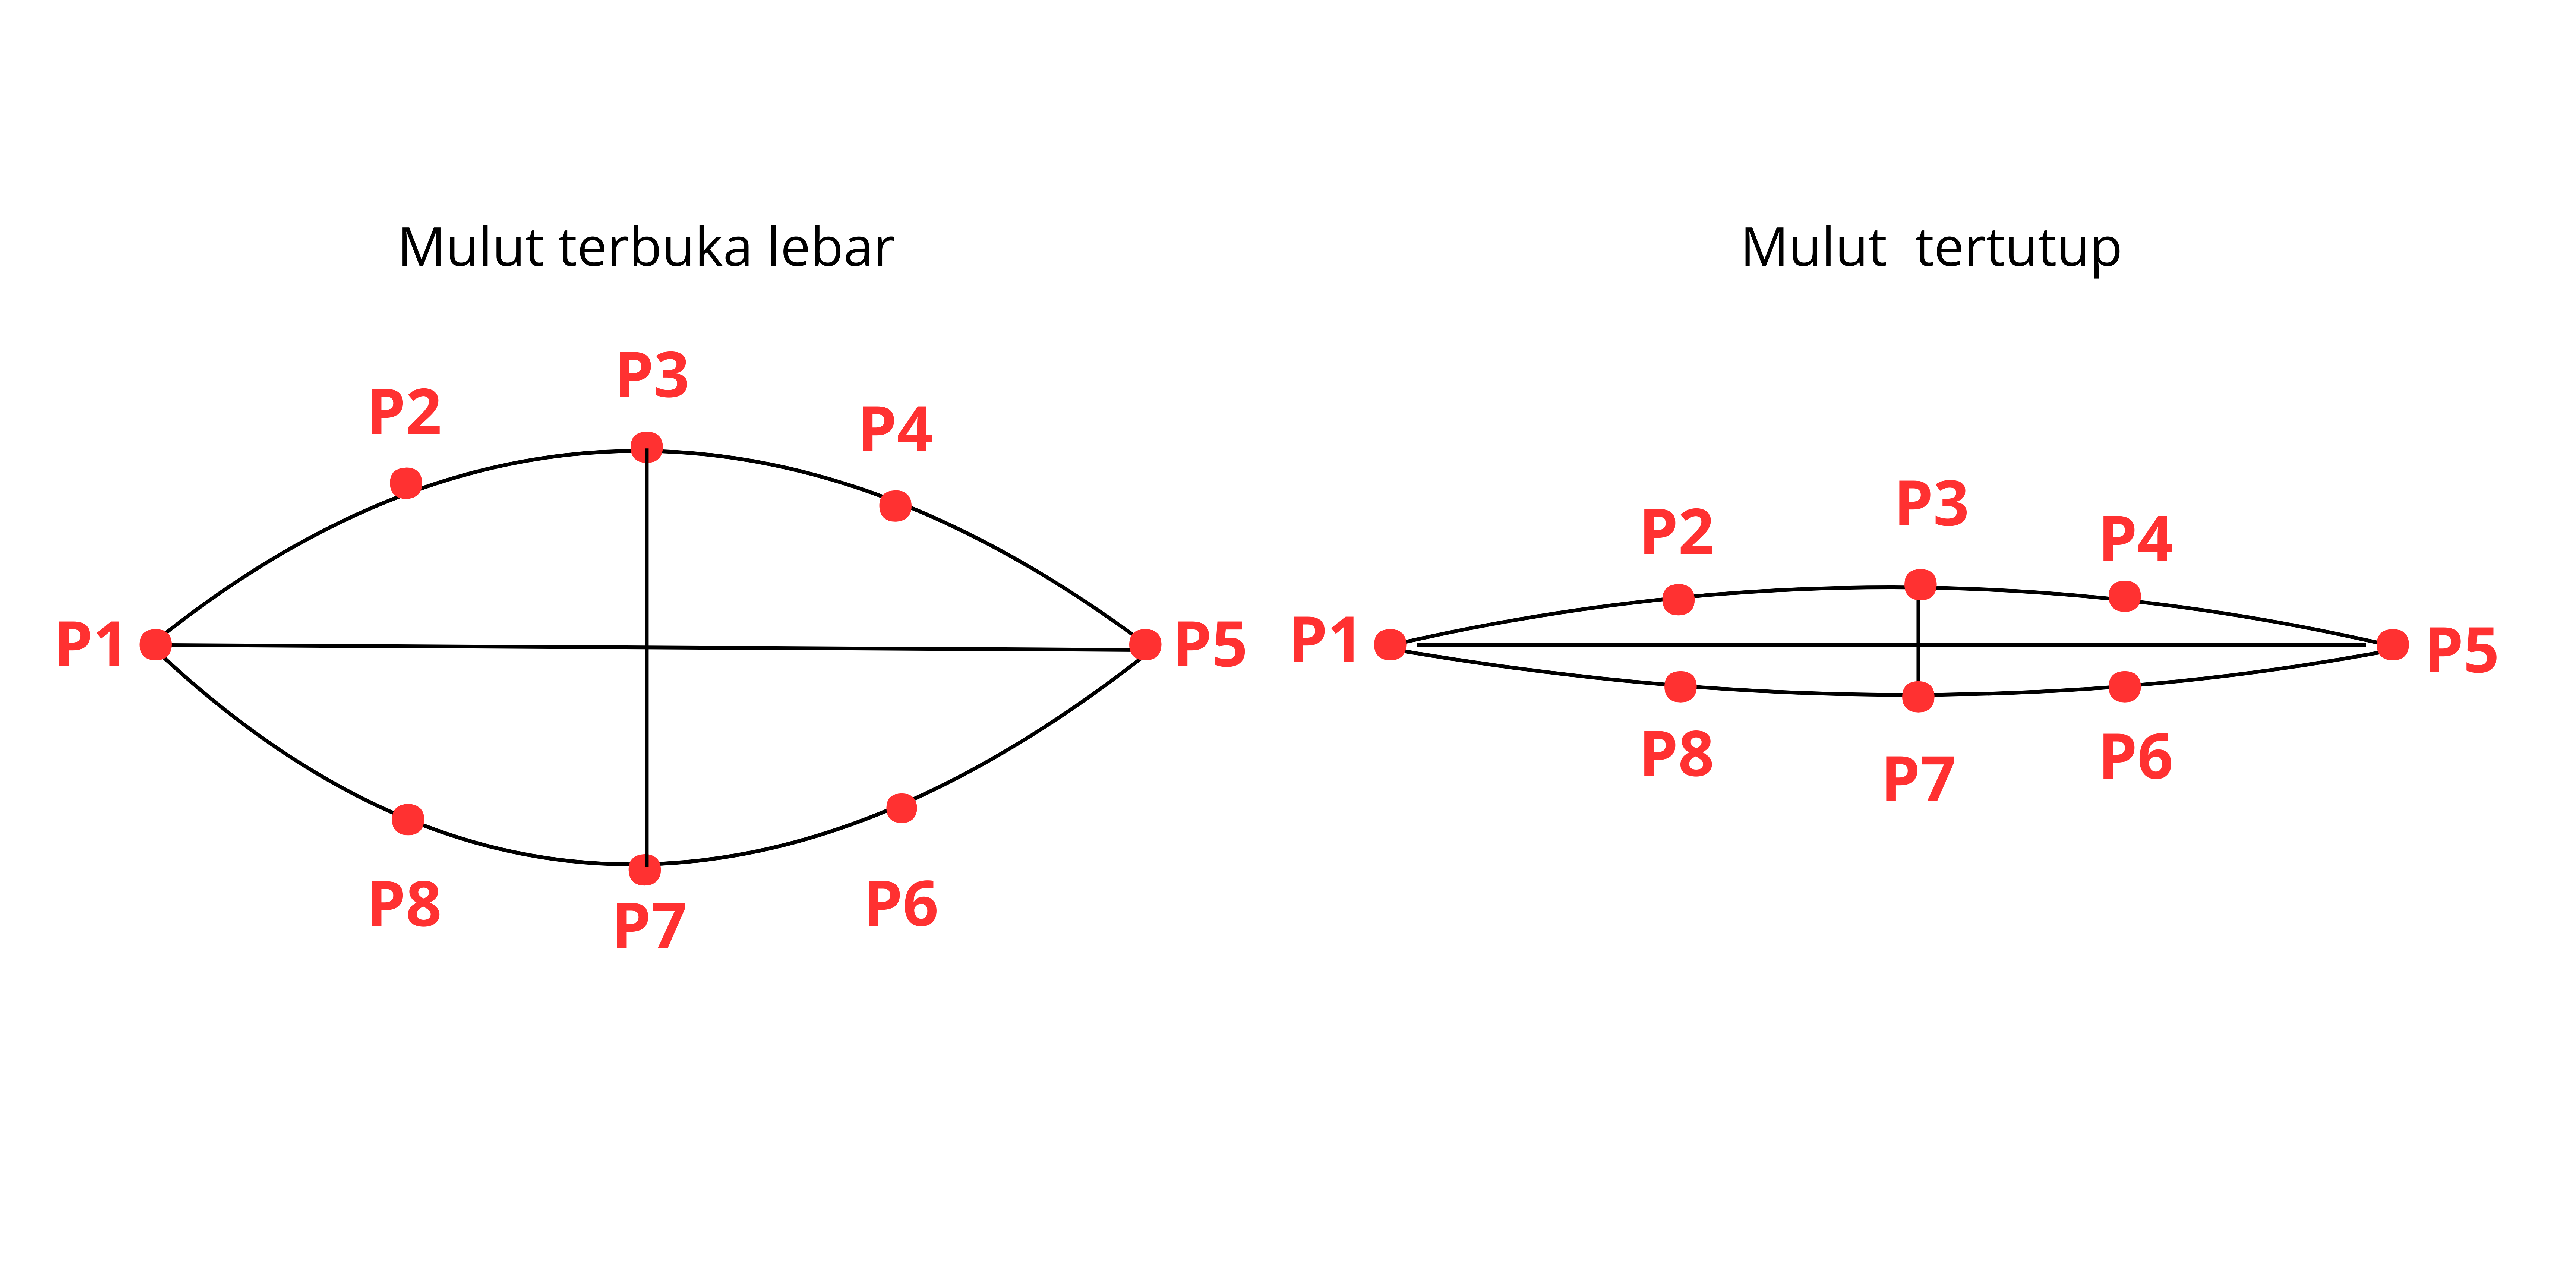
\includegraphics[width=0.8\textwidth]{figures/bab2/mar.png}
      \caption{Ilustrasi Perhitungan Nilai MAR}
      \label{Ilustrasi Perhitungan Nilai MAR}
    \end{figure}

     \begin{equation}
    \label{rumus mar}
    \text{MAR} = \frac{\| \vec{p}_2 - \vec{p}_8 \| + \| \vec{p}_3 - \vec{p}_7 \| + \| \vec{p}_4 - \vec{p}_6 \| }{3 \| \vec{p}_5 - \vec{p}_1 \|}
\end{equation}


      \textbf{Keterangan:}
      
    \begin{align*}
        \vec{p}_i & : \text{Vektor posisi dari titik ke-i} \\
        \|\vec{p}_2 - \vec{p}_8\| & : \text{Jarak antara titik } \vec{p}_2 \text{ dan } \vec{p}_8 \\
        \|\vec{p}_3 - \vec{p}_7\| & : \text{Jarak antara titik } \vec{p}_3 \text{ dan } \vec{p}_7 \\
        \|\vec{p}_4 - \vec{p}_6\| & : \text{Jarak antara titik } \vec{p}_4 \text{ dan } \vec{p}_6 \\
        \|\vec{p}_5 - \vec{p}_1\| & : \text{Jarak antara titik } \vec{p}_5 \text{ dan } \vec{p}_1 \\
    \end{align*}



    

\section{\textit{Convolutional Neural Network} (CNN)}

    \textit{Convolutional Neural Network} (CNN) adalah sub tipe \textit{Artificial Neural Network} (ANN) yang
     dibuat khusus untuk mengatasi tantangan terkait data dua dimensi (2D). \textit{Convolutional Neural Network}
      (CNN) menjalani proses pembelajaran berdasarkan data pelatihan yang diberikan. Mirip dengan jaringan saraf
       manusia ketika mencoba untuk memahami atau mengenali sesuatu, proses pembelajaran ini menghasilkan pola
        yang sesuai. Selanjutnya, setelah mengekstraksi data fitur dari kumpulan data pelatihan, data tersebut
         dapat diterapkan untuk mengatasi masalah klasifikasi \cite{Alzubaidi2021}. 
    
  \begin{figure}[H]
      \centering
      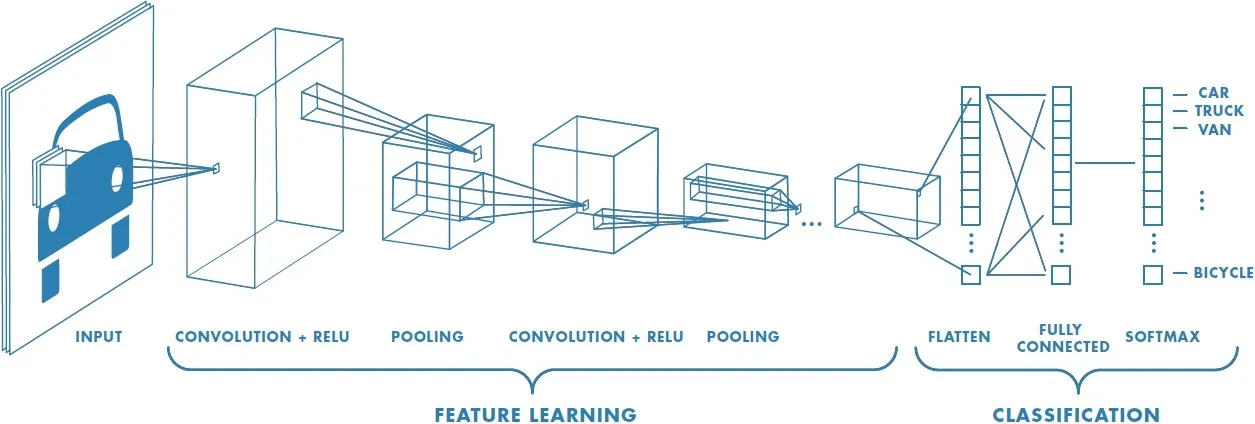
\includegraphics[width=1\textwidth]{figures/bab2/arsitektur cnn.jpg}
      \caption{Arsitektur \textit{Convolutional Neural Network} (CNN) \cite{Prabhu}}
      \label{Arsitektur CNN}
    
    \end{figure}

    Secara garis besar proses pada \textit{Convolutional Neural Network} (CNN) terbagi menjadi dua garis besar yaitu \textit{feature learning} dan \textit{classification}. Pada \textit{input layer} terdapat nilai piksel dan jumlah chanel dari gambar yang dimasukkan, Proses \textit{convolution} menghasilkan \textit{feature map} 
    yang diperoleh dengan menerapkan \textit{filter} berupa matriks.  Di sini, Nilai \textit{feature map} diubah berdasarkan \textit{activation function} yang digunakan seperti ReLU, softmax dan lain-lain. Setelah melewati berbagai proses selanjutkan digunakan \textit{pooling layer} yang bertujuan untuk mengurangi resolusi gambar, namun tidak menghilangkan informasi penting yang dimiliki. Sehingga hal ini dapat mengurangi jumlah parameter dan mempercepat proses klasifikasi. 

    Pada lapisan terakhir terdapat \textit{fully connected layer} dimana semua neuron dari lapisan sebelumnya terhubung 
    pada neuron lapisan berikutnya. Lapisan yang terhubung pada \textit{fully connected layer} sebelumnya telah berubah 
    berubah mejadi data satu dimensi yang disebut dengan \textit{flatten}. \textit{Layer}
    menggunakan semua nilai dan fitur yang telah dipelajari untuk membuat sebuah keputusan sesuai dengan kelas yang telah 
    kita defenisikan sebelumnya. Istilah pada \textit{Convolutional Neural Network} (CNN) akan dibahas di bagian berikut. 


\section{\textit{Layer}}

Pada \textit{Convolutional Neural Network} (CNN) terdapat beberapa \textit{layer} atau lapisan yang disusun 
menjadi beberapa blok. \textit{Layer} pada setiap blok ini berfungsi untuk melakukan proses pengolahan data, 
untuk lebih detailnya dijelaskan pada bagian selanjutnya.


\subsection{\textit{Convolution}}

    Dalam jaringan CNN, lapisan \textit{input} berfungsi sebagai tahap awal yang menerima gambar, sementara lapisan \textit{output} menghasilkan label hasil prediksi. Salah satu tahap penting dalam ekstraksi fitur adalah penggunaan \textit{convolution layer}, yang diposisikan di awal untuk menerima \textit{input} dalam bentuk gambar. \textit{Convolution} merupakan jenis operasi linear khusus dan biasanya menjadi lapisan
    pertama pada model CNN yang disebut sebagai \textit{convolution layer}. Operasi pada
    \textit{convolution} berguna untuk mengubah suatu fungsi menjadi fungsi yang lain. Proses \textit{convolution} akan melakukan konversi
    beberapa data yang telah diinisialisasikan melalui \textit{kernel} kemudian ditangkap
    menjadi ukuran \textit{stride} yang telah ditetapkan.
    Operasi yang dilakukan pada lapisan ini mirip dengan operasi konvolusi, yang melibatkan penggabungan berbagai nilai piksel lokal melalui \textit{filter linier}. \textit{Filter} ini berfungsi sebagai reseptor atau penerima neuron. Lapisan yang mendasari arsitektur CNN dirancang untuk mengekstrak fitur atau informasi dari gambar yang diberikan. Berikut ilustrasi proses pergeseran pada \textit{convolution layer} yang di tujukan pada Gambar \ref{Ilustrasi Proses Pergeseran Filter Pada Convolutional Layer} berikut \cite{Dewi2018}.

  \begin{figure}[H]
      \centering
      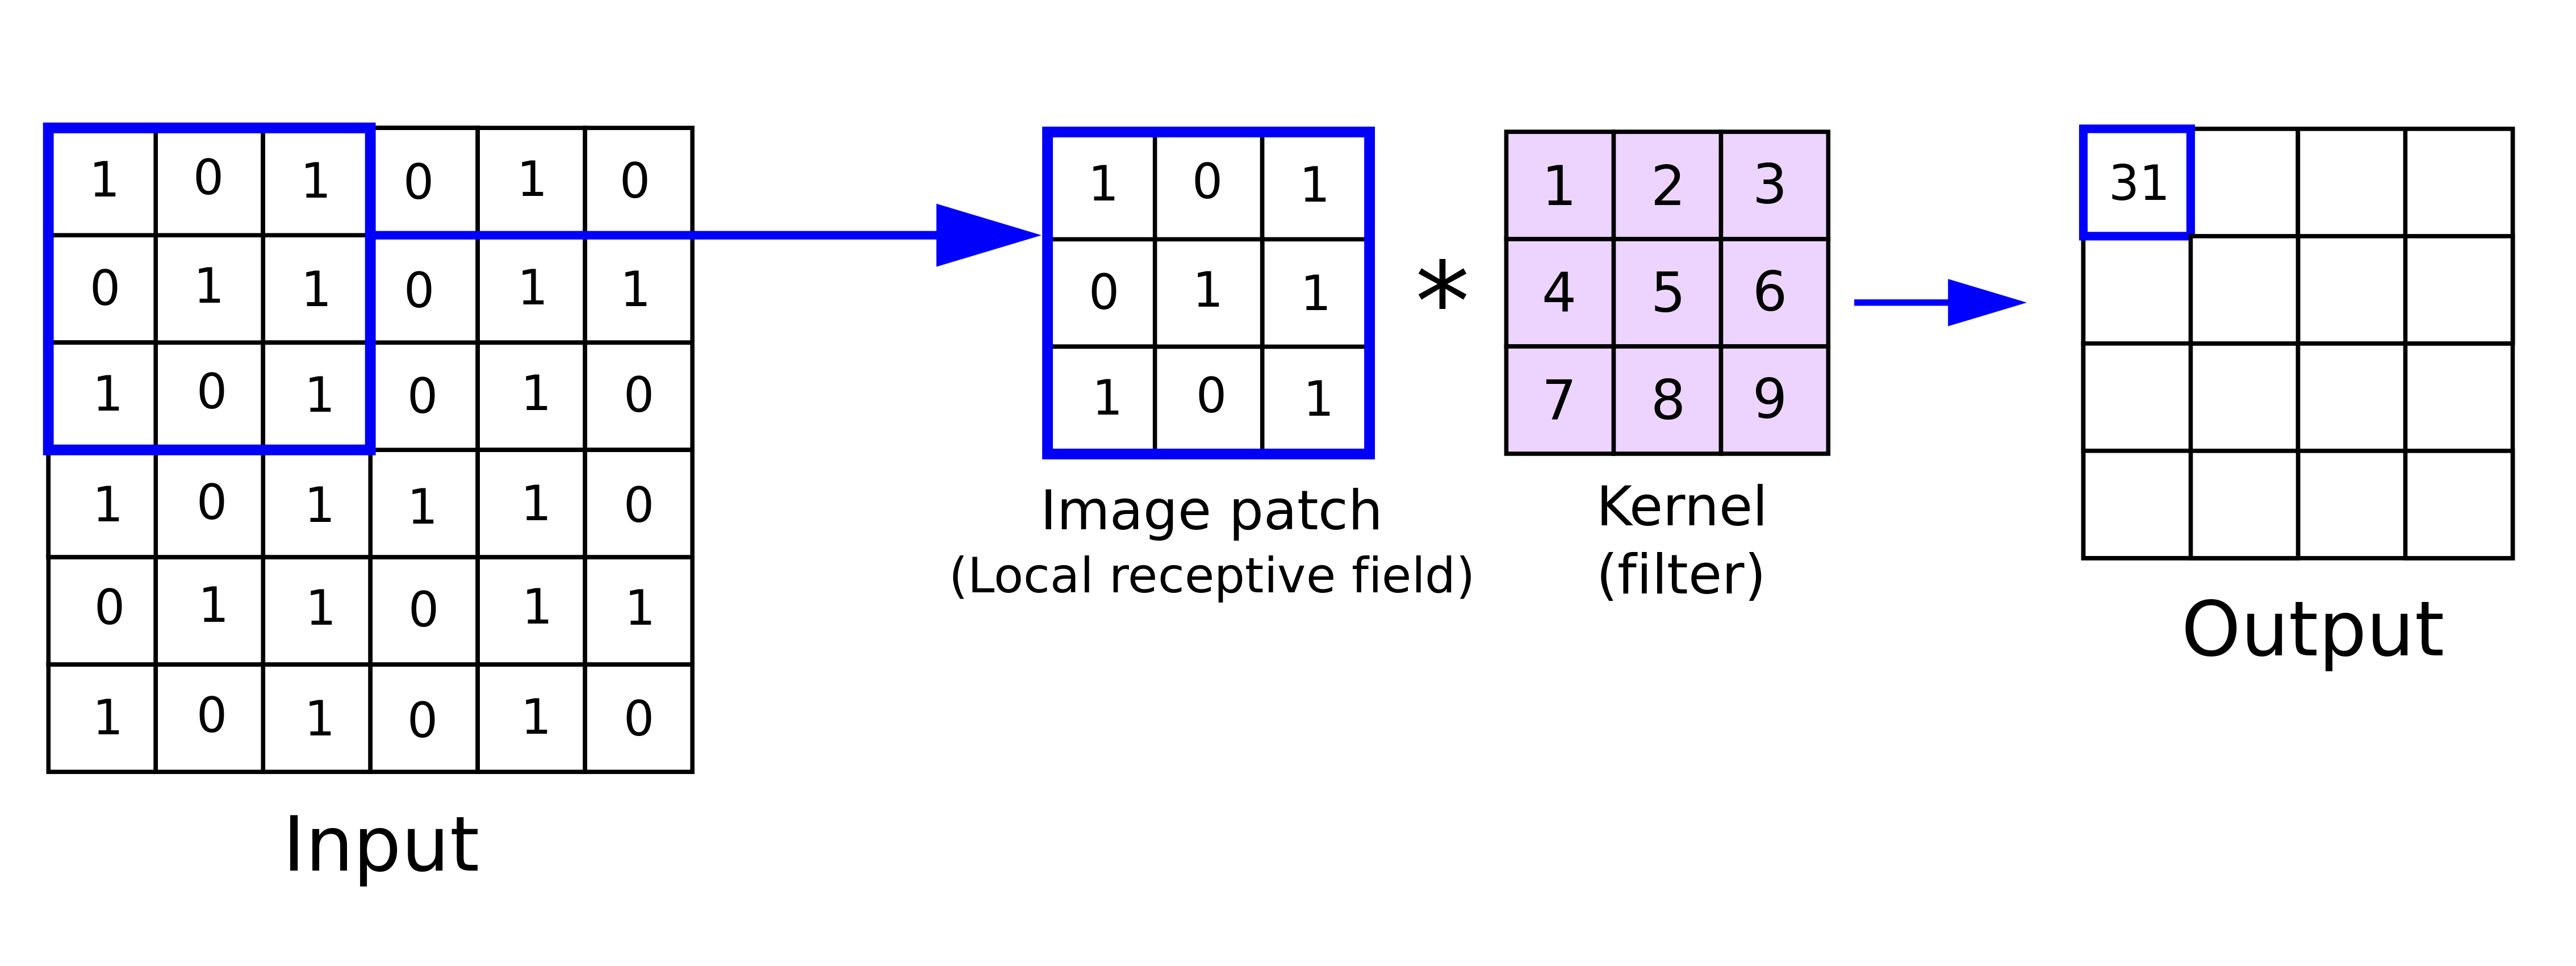
\includegraphics[width=0.8\textwidth]{figures/bab2/cnn.png}
      \caption{Ilustrasi Proses Pergeseran \textit{Filter} \cite{Reynolds}}
      \label{Ilustrasi Proses Pergeseran Filter Pada Convolutional Layer}
    
 \end{figure}


\subsection{\textit{Maxpooling}}

    Lapisan \textit{max pooling} bertanggung jawab untuk menangani matriks \textit{output} dari lapisan sebelumnya, mengurangi ukuran gambar sambil mempertahankan nilai fitur yang penting. Hal ini dilakukan dengan memilih nilai maksimum dari \textit{output} yang dihasilkan oleh lapisan sebelumnya. Pendekatan ini memungkinkan model untuk melakukan proses generalisasi dengan cepat \cite{Gholamalinezhad2020, Nagi2011MaxpoolingCN}. Ilustrasi dari proses \textit{max pooling} ditampilkan pada Gambar \ref{Proses Pada Max Pooling Layer} berikut.


    \begin{figure}[H]
      \centering
      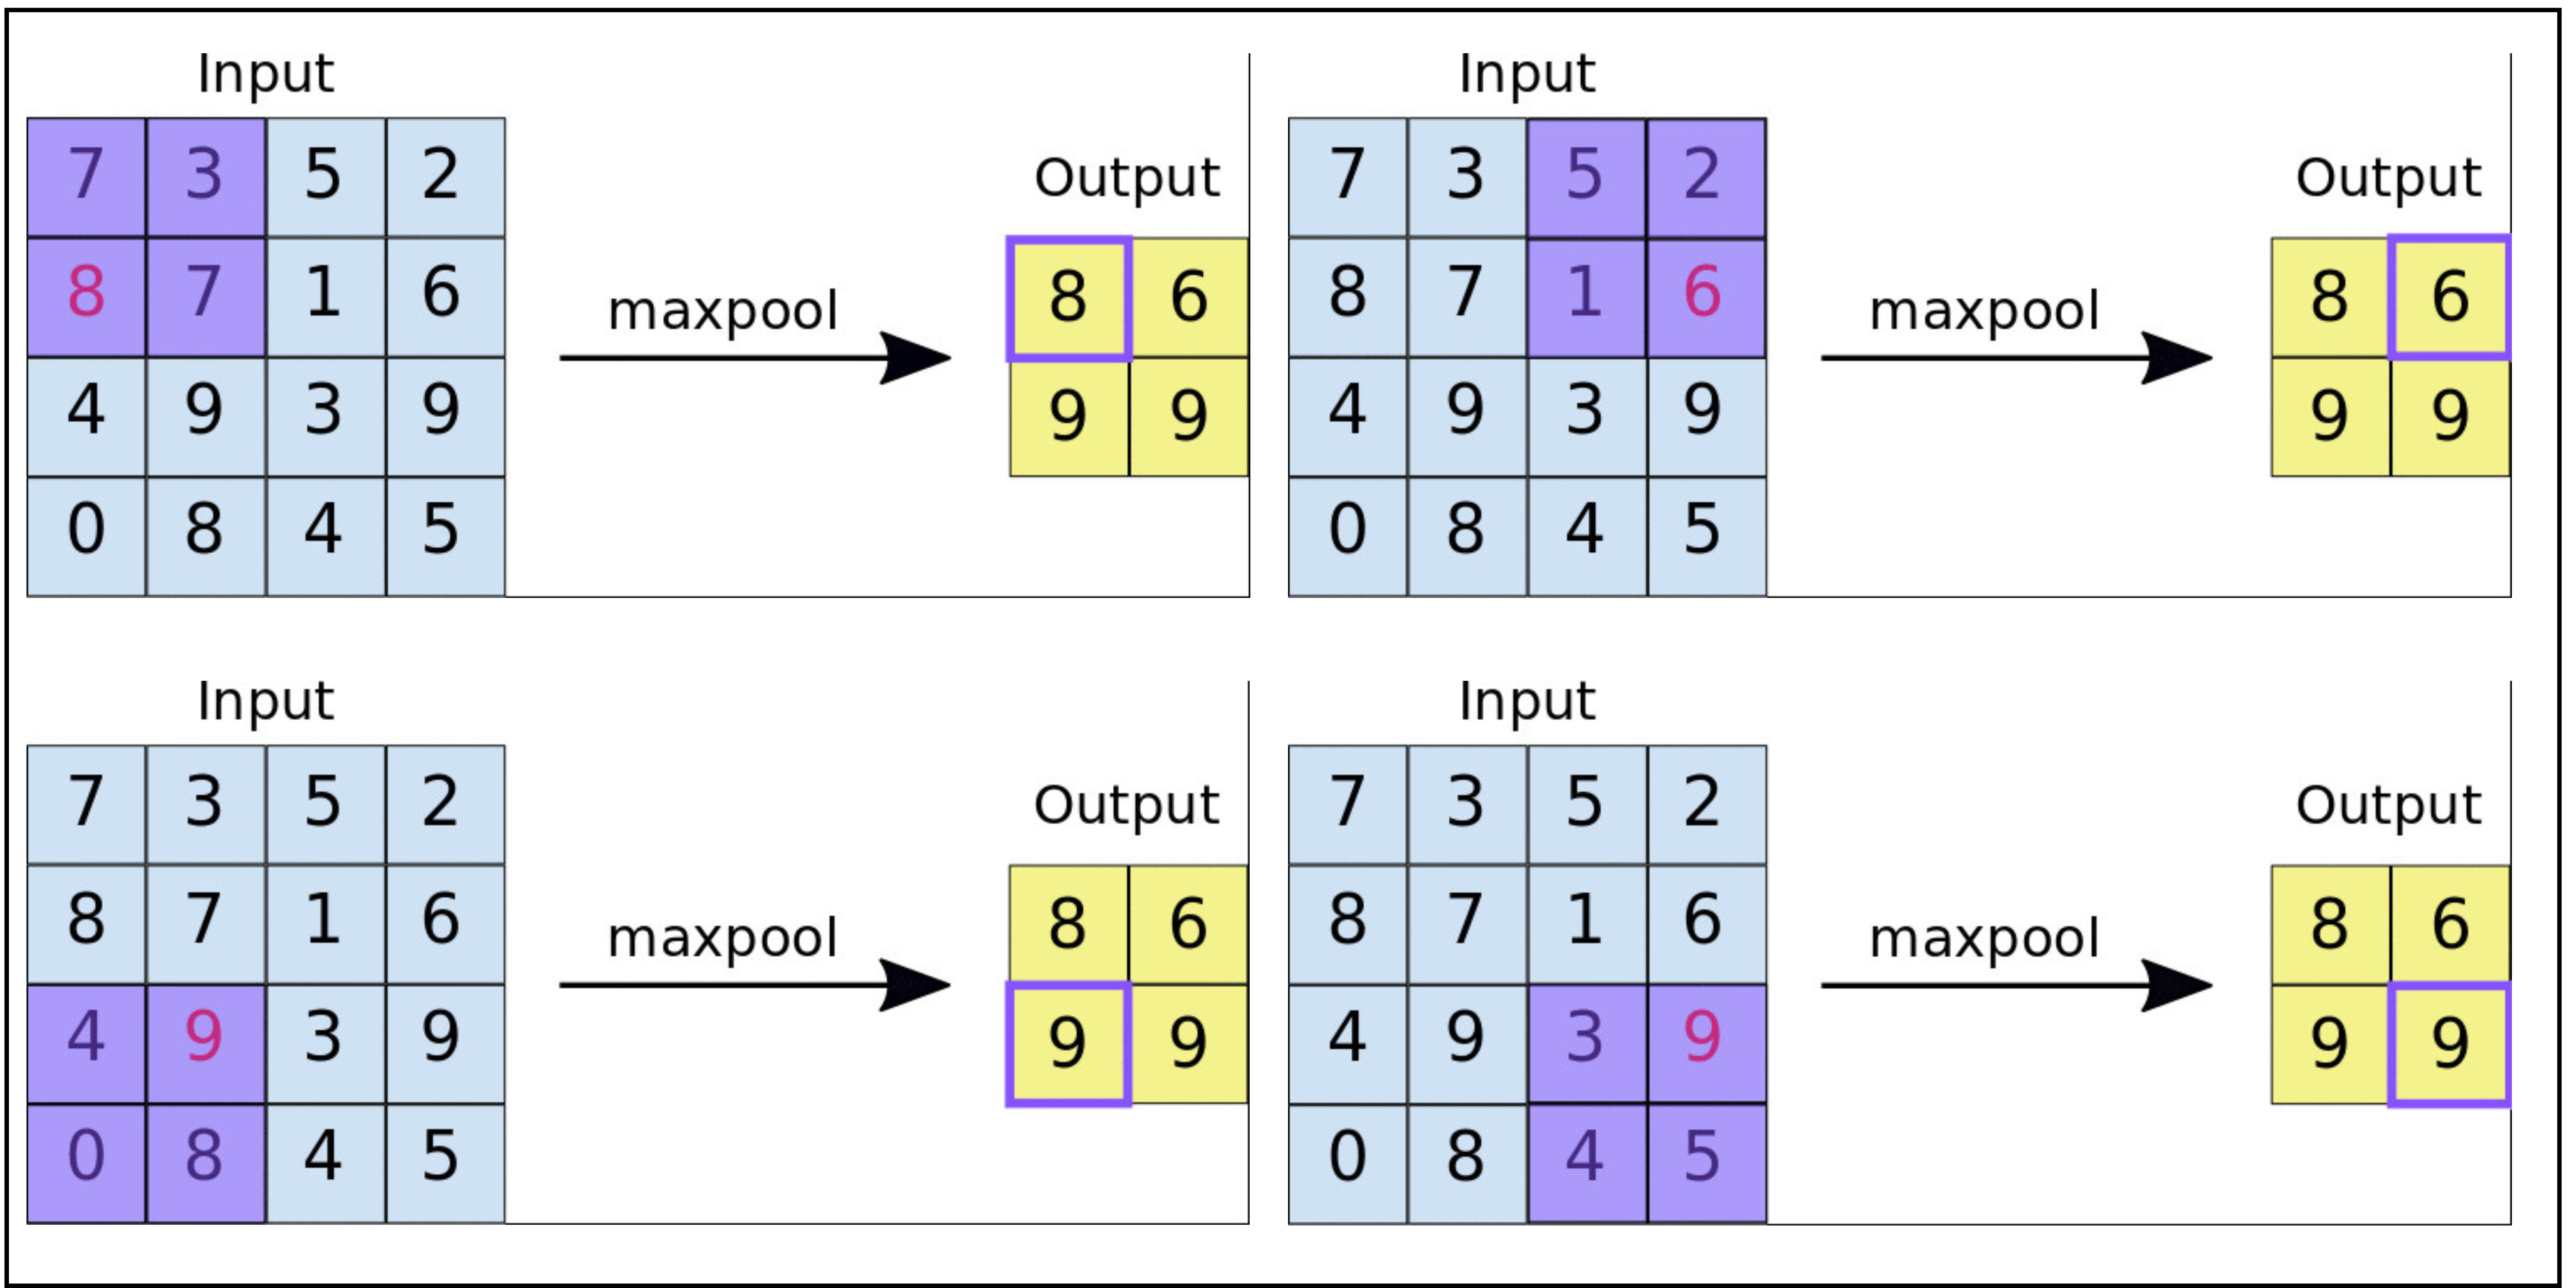
\includegraphics[width=0.75\textwidth]{figures/bab2/pool.png}
      \caption{Proses Pada \textit{Max Pooling Layer} \cite{fiki}}
      \label{Proses Pada Max Pooling Layer}

    
    \end{figure}

\subsection{\textit{Dropout}}

    Banyak lapisan tersembunyi yang biasanya disertakan dalam model \textit{deep learning}, yang membuatnya lebih mudah untuk memahami interaksi yang kompleks antara \textit{input} dan \textit{output}. \textit{Overfitting} adalah masalah yang umum terjadi meskipun ada manfaatnya, terutama pada dataset yang kecil \cite{Srivastava2014}. Untuk mengatasi hal ini, banyak strategi yang telah dikembangkan salah satunya adalah \textit{dropout}. Selain mencegah \textit{overfitting}, lapisan \textit{dropout} secara efektif menggabungkan beberapa jaringan saraf yang terhubung. Hal ini dilakukan dengan menggabungkan lapisan tersembunyi dengan lapisan lain sambil menghapusnya secara bebas dan sesaat \cite{Srivastava2014}. Pada Gambar \ref{Proses Pada Dropout Layer} berikut menunjukkan proses \textit{dropout layer}.

    \begin{figure}[H]
      \centering
      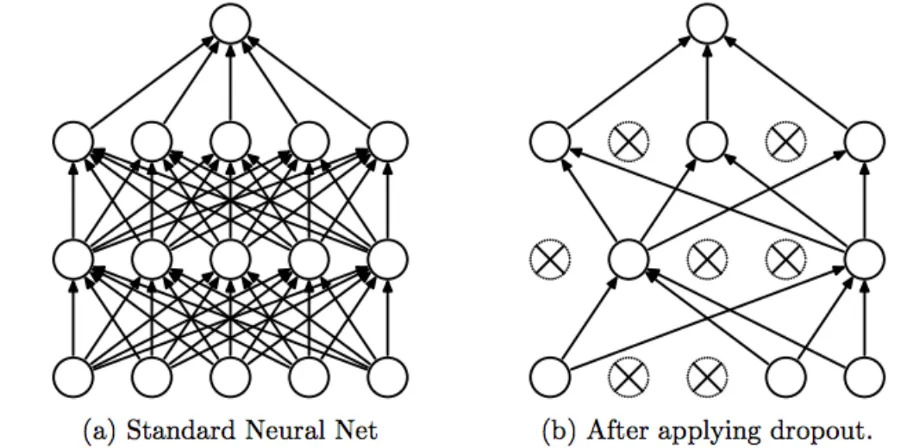
\includegraphics[width=0.70\textwidth]{figures/bab2/drop out.jpg}
      \caption{Proses Pada \textit{Dropout Layer} \cite{ida}}
      \label{Proses Pada Dropout Layer}
    
    \end{figure} 

    
\subsection{\textit{Fully Conected}}

    Lapisan yang terhubung sepenuhnya, juga dikenal sebagai \textit{Multi-Layer Perceptron} (MLP), membangun koneksi antara semua neuron aktivasi di lapisan sebelumnya dan lapisan berikutnya. Lapisan ini mengubah peta fitur yang disajikan sebagai \textit{array} multidimensi menjadi vektor melalui proses perataan, memastikan bahwa setiap aktivasi dari lapisan sebelumnya terhubung secara efektif ke lapisan berikutnya. Umumnya digunakan dalam MLP untuk klasifikasi data, lapisan terhubung sepenuhnya berbeda dari lapisan \textit{convolutional} karena neuron-nya terhubung ke seluruh masukan, menyerupai struktur jaringan saraf manusia yang saling berhubungan. Terlepas dari perbedaan ini, kedua lapisan menjalankan operasi perkalian matriks titik dalam prosesnya \cite{Dewi2018}.

    





\section{\textit{Hyperparameter}}

    \textit{Hyperparameter} dalam CNN merupakan parameter yang tidak secara langsung dipelajari oleh model selama proses \textit{training}. Parameter-parameter ini perlu ditentukan sebelum proses \textit{training} dan memiliki pengaruh signifikan terhadap performa akhir model. Pemilihan nilai \textit{hyperparameter} yang tepat merupakan langkah krusial dalam mengoptimalkan performa CNN.

 \subsection{\textit{Padding}}


    Salah satu parameter dalam CNN adalah \textit{padding}, juga dikenal sebagai \textit{zero padding}, menentukan berapa banyak piksel dengan nilai nol yang ditambahkan ke kedua sisi gambar sebagai masukan. Untuk mengontrol dimensi keluaran di lapisan konvolusi atau peta fitur, \textit{padding} diterapkan. Untuk mengekstrak informasi tambahan, dimensi dimodifikasi untuk mencegah penurunan tajam dalam ukuran dimensi. Secara matematis, untuk menentukan ukuran dimensi keluaran atau peta fitur akhir dapat menggunakan Persamaan \ref{Rumus besaran feature map} \cite{hakim2018implementasi} berikut.
    \begin{equation}
        \begin{aligned}
          o = \left( \frac{i + 2p - k}{s} \right) + 1
      \end{aligned}\label{Rumus besaran feature map}
    \end{equation}



    \textbf{Keterangan:}
        \begin{align*}
        o & : \text{Dimensi luaran} \\
        i & : \text{Dimensi masukan} \\
        k & : \text{Besar dimensi \textit{kernel} atau \textit{filter}} \\
        p & : \text{Nilai \textit{padding}} \\
        s & : \text{Nilai \textit{stride}}
        \end{align*}
        


\subsection{\textit{Stride}}

    \textit{Stride} berfungsi sebagai parameter yang menunjukkan sejauh mana \textit{filter} menggerakkan piksel gambar dalam arah horizontal dan vertikal. Saat ukuran langkah diatur ke satu piksel, \textit{filter} akan bergeser sebesar satu piksel di seluruh gambar. Ukuran langkah berbanding terbalik dengan tingkat informasi detail yang dapat diekstraksi dari suatu gambar, ukuran langkah yang lebih kecil memungkinkan penangkapan informasi yang lebih detail, sedangkan ukuran langkah yang lebih besar memberikan lebih sedikit detail \cite{Dewi2018}.

\subsection{\textit{Activation Function}}

\textit{Activation function} adalah sebuah fungsi yang menentukan apakah sebuah neuron akan menjadi aktif atau tidak. Ada banyak jenis \textit{activation function}, namun pada penelitian ini hanya digunakan tiga jenis, yaitu \textit{Rectified Linear Unit} (ReLU), \textit{sigmoid }dan \textit{softmax}.



\subsubsection{\textit{Rectified Linear Unit}}
    \textit{Rectified Linear Unit} (ReLU) adalah \textit{activation function} yang mampu mengubah nilai negatif menjadi nilai yang lebih besar atau sama dengan nol. Secara matematis, ReLU diwakili oleh rumus dalam Persamaan \ref{Aktifasi Fungsi ReLU}, di mana variabel x mewakili \textit{neuron} \textit{input} dan dikenal sebagai fungsi \textit{ramp}. Jika \textit{input} menghasilkan nilai yang lebih besar dari nol, \textit{output} yang dihasilkan sama dengan \textit{input} yang diberikan. ReLU digunakan secara luas dan telah menunjukkan proses pelatihan yang lebih cepat untuk jaringan yang besar \cite{Dewi2018}.


    \begin{equation}
        \begin{aligned}
            f(x) = \max(x, 0)
        \end{aligned}\label{Aktifasi Fungsi ReLU}
    \end{equation}



\subsubsection{\textit{Softmax Classifier}}

    Salah satu jenis fungsi logistik yang merepresentasikan distribusi satu kategori dalam kaitannya dengan kategori lainnya dan menghitung probabilitas adalah fungsi \textit{softmax}. Fungsi ini membantu menentukan ke dalam kelas atau kategori mana suatu \textit{input} termasuk. \textit{Softmax} banyak digunakan dalam klasifikasi regresi logistik \textit{multinomial} dan analisis diskriminan linier multikelas. Ini menghasilkan hasil yang lebih mudah dipahami daripada algoritma terkait. Hal ini disebabkan oleh sifat \textit{intuitif} dari \textit{output} probabilitas \textit{softmax }yang berkisar antara 0 hingga 1 dan dijumlahkan hingga 1 \cite{Zhang2019}.

        \begin{equation}
            Softmax(z)_i= \frac{e^{z_i}}{\sum_{j=1}^{n} e^{z_j}}
        \end{equation}

     \textbf{Keterangan:}
        

        \begin{align*}
            \text{Softmax}(z)_i &: \text{Nilai peluang untuk elemen ke-}i \\
            z_i &: \text{ nilai \textit{input} x untuk elemen ke-i} \\
            n &: \text{Jumlah total kelas}
        \end{align*}
        



\subsubsection{\textit{Sigmoid}}
    \textit{Activation function} \textit{sigmoid}, juga dikenal sebagai fungsi logistik, adalah fungsi non-linear umum yang digunakan dalam jaringan saraf tiruan. Fungsi ini memetakan nilai \textit{input} menjadi rentang antara 0 dan 1, dan sering digunakan untuk memodelkan probabilitas atau tingkat kepastian. Secara matematis, \textit{activation function} \textit{sigmoid} di definisikan pada Persamaan  \ref{Aktifasi Fungsi Sigmoid} berikut.

    \begin{equation}
        \begin{aligned}
            f(x) = \frac{1}{1 + e^{-x}}
        \end{aligned}\label{Aktifasi Fungsi Sigmoid}
    \end{equation}

     \textbf{Keterangan:}
     
        \begin{align*}
        x & : \text{nilai \textit{input}} \\
        f(x) & :\text{nilai \textit{output}} 
        \end{align*}

        


\subsection{\textit{Optimizer}}

\textit{Optimizer} adalah algoritma yang digunakan untuk menemukan nilai terbaik dari parameter model. Nilai-nilai ini disebut dengan bobot dan mengarahkan pemrosesan data dan membuat prediksi. Tujuan \textit{optimizer} untuk mengurangi nilai akhir dari fungsi \textit{loss}, yang memberi informasi tentang seberapa baik model membuat prediksi data. \textit{Optimizer} itu melaksanakan tugas dengan secara bertahap. Dengan memperbaharui bobot model berdasarkan gradien \textit{loss function}. Gradien adalah besarnya sebaris yang menyebutkan ke mana nilai harus digeser untuk meminimalkan nilai \textit{loss}. Dengan mengikuti instruksi ini, \textit{optimizer} memperbarui nilai bobot yang meminimalkan nilai \textit{loss} dan meningkatkan akurasi model \cite{ruder2017overview}.



\subsubsection{\textit{Stochastic Gradient Descent} (SGD)}

SGD merupakan algoritma iteratif yang bertujuan untuk meminimalkan fungsi \textit{loss} dengan memperbarui parameter model secara bertahap.  Pada setiap iterasi, SGD memperbarui parameter ke arah yang berlawanan dengan gradien dari fungsi \textit{loss}.  Gradien menunjukkan arah perubahan parameter yang akan menghasilkan penurunan \textit{loss} terbesar.  Kesederhanaan dan efisiensi komputasi menjadi daya tarik utama SGD, terutama untuk menangani dataset berukuran besar \cite{math11061360}.
Gradient descent menggunakan regresi linier seperti yang diberikan dalam Persamaan \ref{Stochastic Gradient Descent} berikut.

\begin{equation}
\begin{aligned}
    W = \omega - \eta \cdot \nabla Q_i(\omega) \\
    W \leftarrow \eta \cdot \nabla Q(\omega) \\
    Q(\omega) = \ln \sum_i Q_i(\omega) 
    \Rightarrow \nabla Q(\omega) &= \ln \sum_i \nabla Q_i(\omega)
\end{aligned}
\label{Stochastic Gradient Descent}
\end{equation}
     \textbf{Keterangan:}
     
     \begin{align*}
    W & : \text{Parameter model yang akan diperbarui} \\
    \omega & : \text{Nilai parameter } W \text{ saat ini} \\
    \eta & : \text{\textit{Learning rate}} \\
    Q_i(\omega) & : \text{Nilai fungsi } Q_i \text{ untuk contoh data ke-}i \\
    Q(\omega) & : \text{Nilai rata-rata fungsi } Q_i \text{ untuk semua contoh data}
\end{align*}


    

\subsubsection{\textit{Adaptive Moment Estimation} (Adam)}
Adam didesain untuk mengatasi kekurangan \textit{Stochastic Gradient Descent} (SGD), \textit{optimizer} klasik yang terkenal dengan lambat konvergensinya dan sensitivitasnya terhadap \textit{learning rate}.  Keunggulan utama Adam terletak pada kemampuannya untuk menyesuaikan \textit{learning rate} secara individual untuk setiap parameter (bobot) dalam model.  Hal ini dicapai melalui estimasi momen pertama (\textit{mean}) dan kedua (\textit{variance}) dari gradien, yang membantu Adam untuk mengatasi masalah fluktuasi gradien dan mencapai solusi optimal dengan lebih cepat \cite{miranda2020convolutional}.

    \begin{equation}
    \begin{aligned}
        x_t &= \delta_1 \cdot x_{t-1} - (1 - \delta_1) \cdot g_t \\
        y_t &= \delta_2 \cdot y_{t-1} - (1 - \delta_2) \cdot g_t^2 \\
        \Delta \omega_t &= -\eta \frac{x_t}{\sqrt{y_t + \epsilon}} \cdot g_t \\
        \omega_{t+1} &= \omega_t + \Delta \omega_t
    \end{aligned}
    \label{Adam}
    \end{equation}

 \textbf{Keterangan:}

    \begin{align*}
    x_t &: \text{Estimasi pertama dari rata-rata gradien pada iterasi ke-t}\\
    y_t &: \text{Estimasi kedua dari rata-rata gradien kedua pada iterasi ke-t}\\
    \omega_t &: \text{\textit{Learning rate} yang disesuaikan pada iterasi ke-t}\\
    g_t &: \text{Gradien dari parameter pada iterasi ke-t}\\
    \delta_1, \delta_2 &: \text{Hyperparameter untuk estimasi pertama dan kedua terhadap gradien baru}\\
    \eta &: \text{\textit{Learning rate}}\\
\end{align*}









    

\section{\textit{Confusion Matrix}}

    Mengevaluasi efektivitas model penilaian melibatkan pemeriksaan parameter kinerja seperti \textit{accuracy}, \textit{precision}, \textit{recall}, dan \textit{F1-Score}. Perhitungan parameter ini memerlukan penggunaan \textit{confusion matrix}, seperti yang digambarkan pada Gambar \ref{Confusion Matrix} \cite{Nurhikmat2018}.

    \begin{figure}[H]
      \centering
      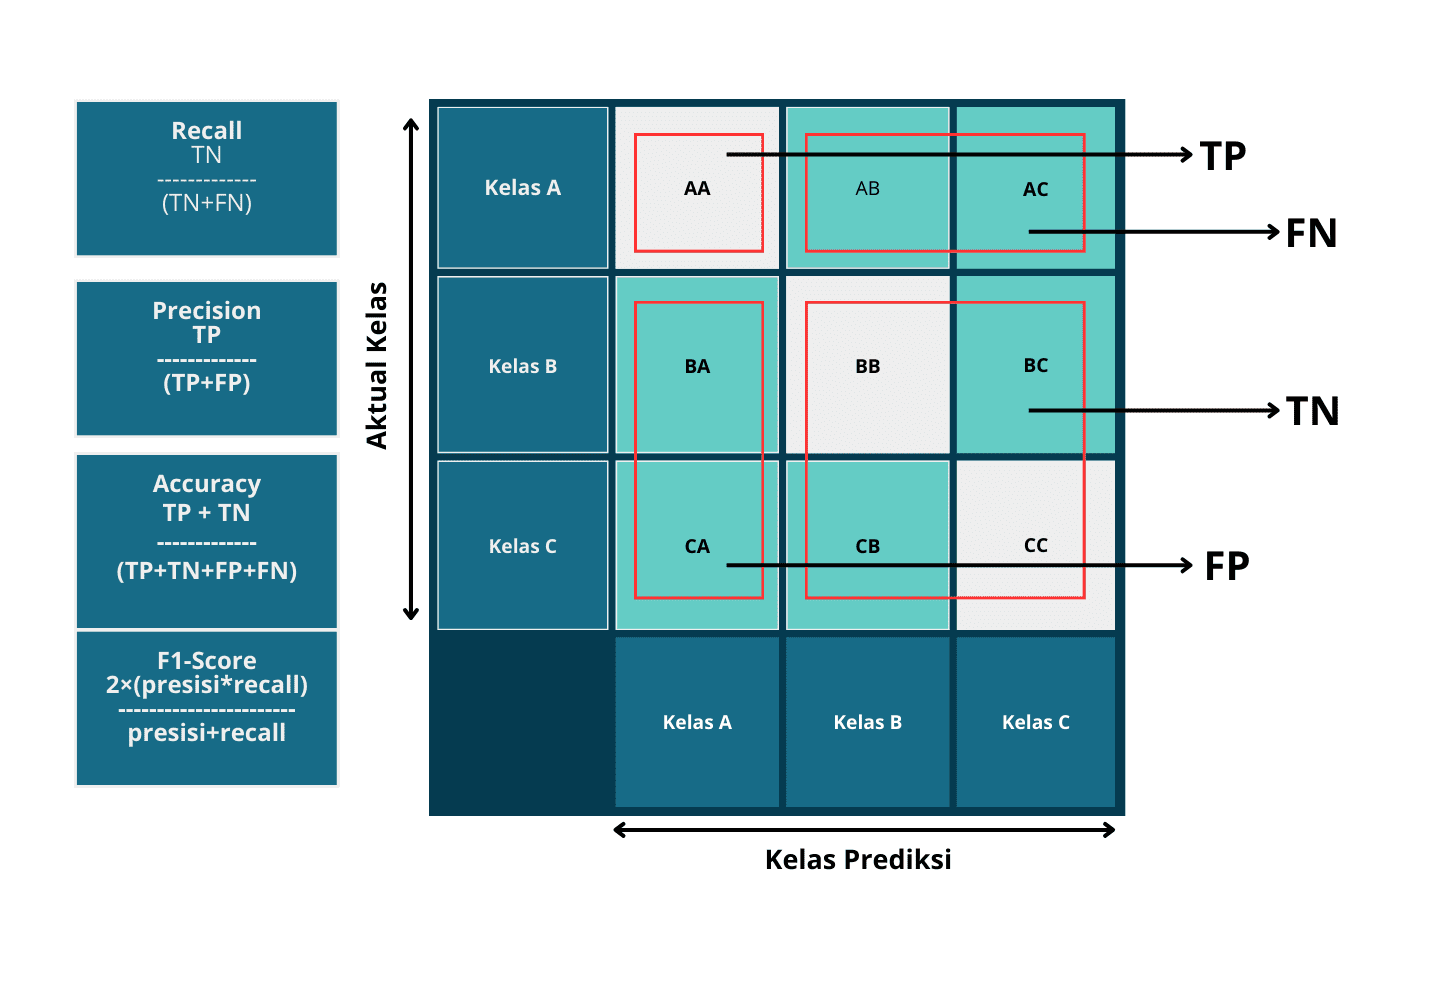
\includegraphics[width=0.75\textwidth]{figures/bab2/confusion matriks.png}
      \caption{\textit{Confusion Matrix}}
      \label{Confusion Matrix}
    
    \end{figure}

    Gambar 2.14 menampilkan empat nilai, yaitu "\textit{True Positive}" (TP), "\textit{False Negative}" (FN), "\textit{False Positive}" (FP), dan "\textit{True Negative}" (TN). Keempat nilai tersebut dapat digunakan untuk menghitung parameter-parameter seperti \textit{accuracy}, \textit{precision}, \textit{recall}, dan \textit{F1-Score} \cite{Nurhikmat2018}.

     \textit{Accuracy} digunakan untuk mengevaluasi sejauh mana model mampu melakukan klasifikasi dengan tepat dengan Persamaan \ref{Accuracy} berikut. 
     
    \begin{equation}
        \begin{aligned}
            \textit{Accuracy} = \frac{\text{TP} + \text{TN}}{\text{TP} + \text{TN} + \text{FN} + \text{FP}}
        \end{aligned}\label{Accuracy}
    \end{equation}


    \textit{Recall} merupakan parameter yang didapat dari jumlah data benar untuk mengukur seberapa baik model dalam mengidentifikasi kelas positif. \textit{Recall} juga dikenal sebagai sensitifitas prediksi dengan Persamaan \ref{Recall} beriikut.

    
    \begin{equation} 
        \begin{aligned}
            \textit{Recall} = \frac{\text{TP}}{\text{TP} + \text{FN}} 
        \end{aligned}\label{Recall}
    \end{equation}

    \textit{Precision} merupakan parameter penilaian yang menghitung jumlah data yang benar antara nilai sebenarnya dengan hasil prediksi model. Digunakan juga untuk mengukur seberapa baik model dalam mengidentifikasi kelas positif dengan menggunkan Persamaan \ref{Precision} berikut.
     \begin{equation}
        \begin{aligned}
            \text{\textit{Precision}} = \frac{\text{TP}}{\text{TP} + \text{FP}}
        \end{aligned}\label{Precision}
    \end{equation}

    \textit{F1-Score} merupakan rata-rata harmonik dari recall dan precision dengan Persamaan \ref{F1-Score}. Secara representasi, jika \textit{F1-Score} punya skor yang baik mengindikasikan bahwa model klasifikasi yang ada memiliki nilai \textit{recall} dan precision yang baik.

     \begin{equation}
        \begin{aligned}
         F1-Score =   2 \times \frac{precision \times recall}{precision + recall}
        \end{aligned}\label{F1-Score}
    \end{equation}

    


    

